\documentclass[english,aspectratio=1610,9pt,helvet,nicetitles]{ICEbeamerTUMCD}
% options: 169, 1610, 43, mathTUMCD, english, german, ngerman, helvet, handout, notes, ruled, nicetitles
% Unknown options are passed to beamer class, e.g., pass t for top alignment of slide content

\newcommand{\PersonTitel}{}
\newcommand{\PersonVorname}{David}
\newcommand{\PersonNachname}{de Andrés Hernández}
\newcommand{\PersonStadt}{Munich}
\newcommand{\PersonAdresse}{%
    Boschetsriederstr. 55A\\%
    81379~\PersonStadt%
}
\newcommand{\PersonTelefon}{@Telefon@}
\newcommand{\PersonEmail}{@E-Mail@}
\newcommand{\PersonWebseite}{@Web@}
% Fakultät:
\newcommand{\FakultaetName}{Department of Electrical and Computer Engineering}
\newcommand{\LehrstuhlName}{Institute for Communications Engineering}

\hyphenation{} % eigene Silbentrennung
%%%%%%%%%%%%%%%%%%%%%%%%%%%%%%%%%%%%%%%%%%%%%%%%%%%%%%%%%%%%%%%%%%%%%%%%%%%%%%%%


\newcommand{\Datum}{\today}


\title{Geometric and Probabilistic Constellation\\ \vspace{0.5cm} Shaping with Autoencoders}
\subtitle{Research Internship} % Comment out if no subtitle wanted
\author{\PersonVorname{} \PersonNachname{}}
\institute[]{Technical University of Munich \\ Institute for Communications Engineering}

% \setlength{\offsetTitle}{1cm} % Adjust spacing between title and header
% \setlength{\authorOffsetTitlepage}{5cm} % Adjust spacing between author and title

% More layouts of notes can be activated by uncommenting the following
% See https://github.com/gdiepen/latexbeamer-handoutWithNotes for all available layouts
% \pgfpagesuselayout{3 on 1 with notes}[a4paper,border shrink=5mm]
\graphicspath {{/home/ddeandres/Projects/internship_pcs/documentation/figs/}}
\usepackage[backend=bibtex,style=ieee-alphabetic,natbib=true, maxcitenames=2]{biblatex} %added
\usepackage{subfigure} %added
\usepackage{tikzscale} %added
\usepackage{physics}
\addbibresource{/home/ddeandres/Projects/internship_pcs/documentation/refs.bib}

\begin{document}
\setlength{\baselineskip}{\PraesentationAbstandAbsatz}
\setlength{\parskip}{\baselineskip}
% \let\thefootnote\relax\footnote
\PraesentationMasterStandard

\PraesentationTitelseite % Fügt die Startseite eon

\begin{frame}{Agenda}
  \begin{enumerate}
  \item Introduction
  	\begin{itemize}
  	\item SNR Gap
  	\item Probabilistic Constellation Shaping
  	\item Geometric Shaping
  	\end{itemize}
  \item Autoencoders
	\begin{itemize}
	\item Challenges
  	\end{itemize}
  \item Contribution
  \begin{itemize}
  	\item First Implementation
  	\item Second Implementation
  \end{itemize}
  \item Conclusions
  \end{enumerate}
\end{frame}


\begin{frame}{Introduction}
  \begin{itemize}
  \item We want to make use of each channel's capacity as efficiently as possible
  $$ C = \max_{p(X): \mathbb{E}[X^2] \leq P} \mathbb{I}(X;Y)$$
  \item The optimal $p(x)$ has only been found for specific channels, such as the AWGN, since knowledge of the channel distribution $p(y|x)$ is required.
  \end{itemize}
  \begin{minipage}{0.5\linewidth}
    % This file was created with tikzplotlib v0.10.1.
\begin{figure}

\centering
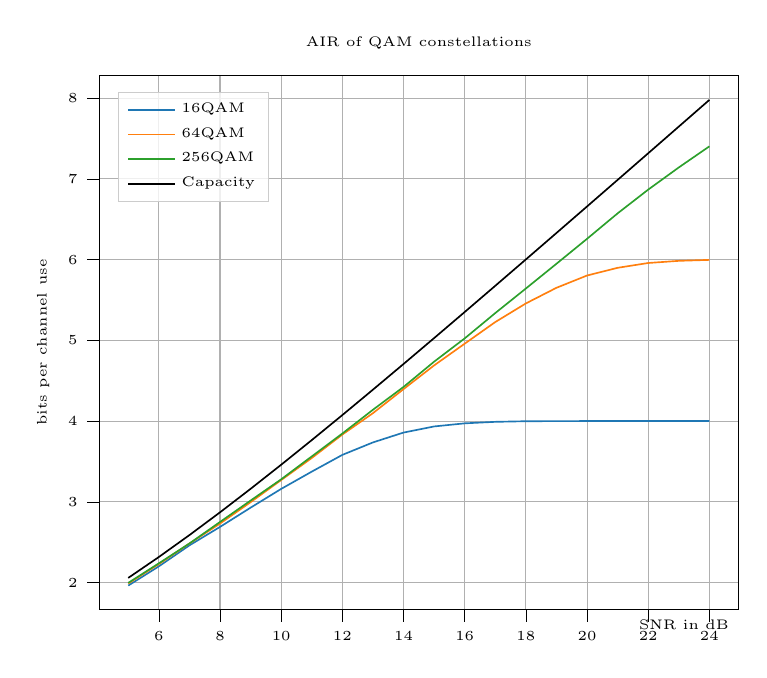
\begin{tikzpicture}[font=\tiny]

\definecolor{darkgray176}{RGB}{176,176,176}
\definecolor{darkorange25512714}{RGB}{255,127,14}
\definecolor{forestgreen4416044}{RGB}{44,160,44}
\definecolor{lightgray204}{RGB}{204,204,204}
\definecolor{steelblue31119180}{RGB}{31,119,180}

\begin{axis}[
width={0.8*\columnwidth},
legend cell align={left},
legend style={
  fill opacity=0.8,
  draw opacity=1,
  text opacity=1,
  at={(0.03,0.97)},
  anchor=north west,
  draw=lightgray204
},
tick align=outside,
tick pos=left,
title={AIR of QAM constellations},
x grid style={darkgray176},
%xlabel near ticks,
xlabel={SNR in dB},
xlabel style= {at={(current axis.right of origin)},anchor=north east},
xmajorgrids,
xmin=4.05, xmax=24.95,
xtick style={color=black},
y grid style={darkgray176},
ylabel near ticks,
ylabel={bits per channel use},
ymajorgrids,
ymin=1.66181892569305, ymax=8.27914714409211,
ytick style={color=black}
]
\addplot [semithick, steelblue31119180]
table {%
5 1.96260657198392
6 2.20057890668296
7 2.46062850232861
8 2.68916771012653
9 2.92754785471189
10 3.16001374864848
11 3.37394207587711
12 3.5813072528598
13 3.73563160246622
14 3.8577293286867
15 3.93341963126162
16 3.9717667139498
17 3.9904851697786
18 3.99800425910086
19 3.99934828256524
20 3.99999626348943
21 3.99999989622735
22 3.99999999998693
23 4
24 4
};
\addlegendentry{16QAM}
\addplot [semithick, darkorange25512714]
table {%
5 1.98831629669083
6 2.22879956645784
7 2.48336412143054
8 2.73062650407162
9 2.99541195560546
10 3.26957522314531
11 3.54252933282761
12 3.83300500758109
13 4.09796073536366
14 4.39583835285265
15 4.68954203431748
16 4.95874540957307
17 5.22667699129876
18 5.45712334725999
19 5.65094798938173
20 5.80274592475937
21 5.8982378661517
22 5.95774486109582
23 5.98445084927041
24 5.99631124611408
};
\addlegendentry{64QAM}
\addplot [semithick, forestgreen4416044]
table {%
5 1.99598808718018
6 2.23808070724083
7 2.4839053353697
8 2.75050198042106
9 3.01563315620481
10 3.27886109483527
11 3.56250118335137
12 3.84593827897624
13 4.14024915520781
14 4.42277376162156
15 4.73577678660621
16 5.02419755486895
17 5.33792085218718
18 5.64198608467194
19 5.94846950741156
20 6.25755400977467
21 6.5729057290541
22 6.86698540504613
23 7.14160828296039
24 7.40282515785071
};
\addlegendentry{256QAM}
\addplot [semithick, black]
table {%
5 2.0573732086068
6 2.31645617962626
7 2.58781437356203
8 2.86978721917029
9 3.16080442391302
10 3.4594316186373
11 3.76439436704286
12 4.07458523490543
13 4.38905896736305
14 4.70702026272884
15 5.02780767335052
16 5.3508761542486
17 5.67577990180488
18 6.00215644400198
19 6.32971245944191
20 6.65821148275179
21 6.98746345895592
22 7.31731600193655
23 7.64764716249041
24 7.97835949780125
};
\addlegendentry{Capacity}
\end{axis}

\end{tikzpicture}
\end{figure}
  \end{minipage}%
  \begin{minipage}{0.5\linewidth}
    % This file was created with tikzplotlib v0.10.1.
\begin{figure}
\centering

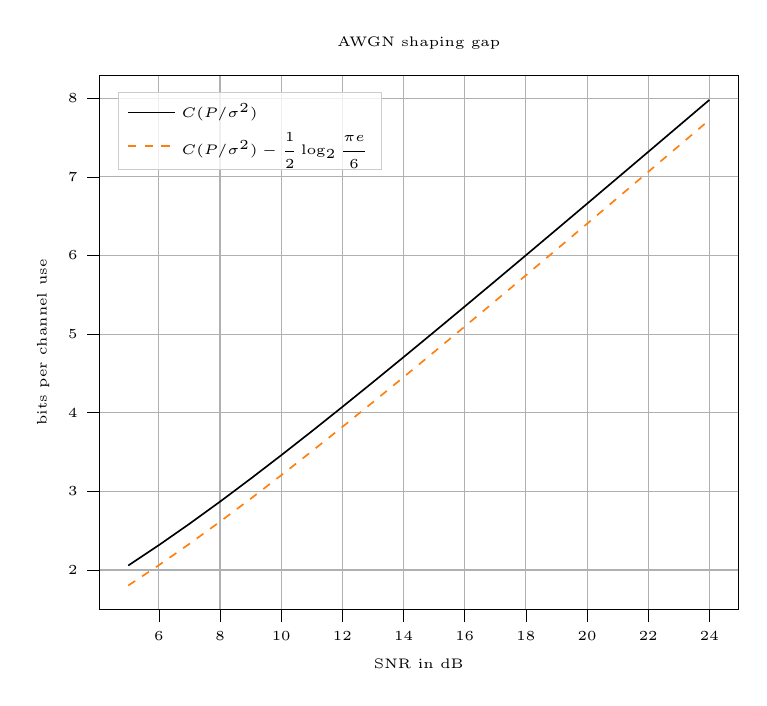
\begin{tikzpicture}[font=\tiny]

\definecolor{darkgray176}{RGB}{176,176,176}
\definecolor{darkorange25512714}{RGB}{255,127,14}
\definecolor{lightgray204}{RGB}{204,204,204}

\begin{axis}[
width={0.8*\columnwidth},
legend cell align={left},
legend style={
  fill opacity=0.8,
  draw opacity=1,
  text opacity=1,
  at={(0.03,0.97)},
  anchor=north west,
  draw=lightgray204
},
tick align=outside,
tick pos=left,
title={AWGN shaping gap},
xlabel near ticks,
x grid style={darkgray176},
xlabel={SNR in dB},
xmajorgrids,
xmin=4.05, xmax=24.95,
xtick style={color=black},
y grid style={darkgray176},
ylabel near ticks,
ylabel={bits per channel use},
ymajorgrids,
ymin=1.49397884258601, ymax=8.28713952900197,
ytick style={color=black}
]
\addplot [semithick, black]
table {%
5 2.0573732086068
6 2.31645617962626
7 2.58781437356203
8 2.86978721917029
9 3.16080442391302
10 3.4594316186373
11 3.76439436704286
12 4.07458523490543
13 4.38905896736305
14 4.70702026272884
15 5.02780767335052
16 5.3508761542486
17 5.67577990180488
18 6.00215644400198
19 6.32971245944191
20 6.65821148275179
21 6.98746345895592
22 7.31731600193655
23 7.64764716249041
24 7.97835949780125
};
\addlegendentry{$C(P/\sigma^2)$}
\addplot [semithick, darkorange25512714, dashed]
table {%
5 1.80275887378673
6 2.0618418448062
7 2.33320003874197
8 2.61517288435022
9 2.90619008909296
10 3.20481728381723
11 3.5097800322228
12 3.81997090008536
13 4.13444463254298
14 4.45240592790877
15 4.77319333853046
16 5.09626181942854
17 5.42116556698482
18 5.74754210918192
19 6.07509812462185
20 6.40359714793173
21 6.73284912413586
22 7.06270166711648
23 7.39303282767034
24 7.72374516298118
};
\addlegendentry{$C(P/\sigma^2) - \dfrac{1}{2}\log_2\dfrac{\pi e}{6}$}
\end{axis}

\end{tikzpicture}
\end{figure}
  \end{minipage}
\end{frame}

\begin{frame}{Closing the SNR Gap}
	\begin{itemize}
	\item ASK and QAM modulation schemes are penalized for two reasons:
	\begin{enumerate}
		\item They use uniform probability densities
		\item The constellation points are equidistant
	\end{enumerate}
	\item Solution 1: Shape the probability of occurrence of the constellation points --- Probabilistic Constellation Shaping
	\item Solution 2: Shape the space location of the constellation points --- Geometric Constellation Shaping
	\begin{figure}
	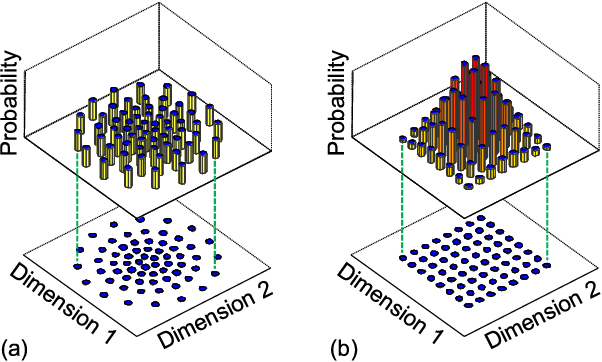
\includegraphics[width=0.4\columnwidth]{ressources/PCS_GCS.png}
	\caption{(a) Probabilistic Constellation Shaping, (b) Geometric Constellation Shaping; \cite{Cho2019ProbabilisticCS}}
	\end{figure}
	\end{itemize}

\end{frame}

\begin{frame}{Why does it makes sense to use ML for this problem?}
\begin{itemize}
\item Finding the constellation parameters when $p(y|x)$ is very complex or unknown can be mathematically untractable
\item NN have the property of being universal function approximators \cite{HORNIK1989359}
\item \citet{O'Shea} pioneered the idea of interpreting the complete communication system as an autoencoder
% e2e optimization of transmitter and receiver
\end{itemize}
\begin{figure}
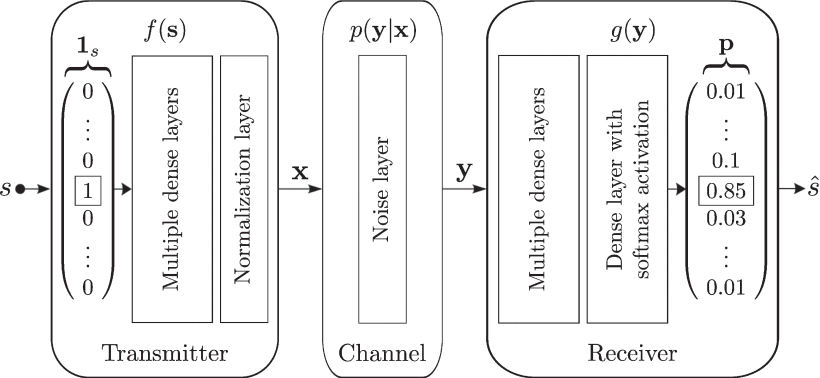
\includegraphics[width=0.5\columnwidth]{ressources/oshea.png}
\caption{Autoencoder architecture proposed by \citep{O'Shea}.}
\end{figure}
\end{frame}

\begin{frame}{Autoencoders}
\begin{itemize}
%\item Autoencoders have been successfully implemented in fields like computer vision or data compression.
\item Idea: transmit a particular representation of the input data so that at the output, it can be reconstructed with minimal error
\item This representations must be robust with respect to the channel impairments (i.e. noise, fading, distortion, etc.) --- bottleneck in the autoencoder jargon
\item The autoencoder is implemented using Feed-forward Neural Networks (FFNN), and the parameters are learned using Stochastic Gradient Descent (SGD)
\end{itemize}
\vspace{-5mm}
\begin{figure}
\centering
\resizebox{!}{11em}{
\tikzset{
    neuron/.style={
		circle,
		draw=black,
		minimum size=0.4cm,
		fill=gray,
	},	
    neuron dark/.style={
		circle,
		draw=black,
		minimum size=0.4cm,
		fill=TUMBlueDark,
	},	
	neuron missing/.style={
		draw=none, 
		fill=white,
		scale=1.0,
		text height=0.3cm,
		execute at begin node=\color{black}$\vdots$
	},
	label/.style = {draw=none, fill=none, rectangle, minimum height=1em, minimum width=1em},
	blockrx/.style = {draw, fill=white, rectangle, minimum height=1.5em, minimum width=6.25em},
	blocktx/.style = {draw, fill=white, rectangle, minimum height=1.5em, minimum width=13em},
	block/.style = {draw, fill=white, rectangle, minimum height=2em, minimum width=10em,rounded corners},
	blockthesis/.style = {draw, fill=gray!20, rectangle, minimum height=1.5em, minimum width=40em,rounded corners},
	block1/.style = {draw, fill=white, rectangle, minimum height=1.5em, minimum width=1.5em,rounded corners},
	tmp/.style  = {coordinate}, 
	sum/.style= {draw, fill=white, circle, node distance=1cm},
	mul/.style= {draw=none, fill=white, circle, node distance=1cm},
	input/.style = {coordinate},
	output/.style= {coordinate},
	pinstyle/.style = {pin edge={to-,thin,black}
	}
}
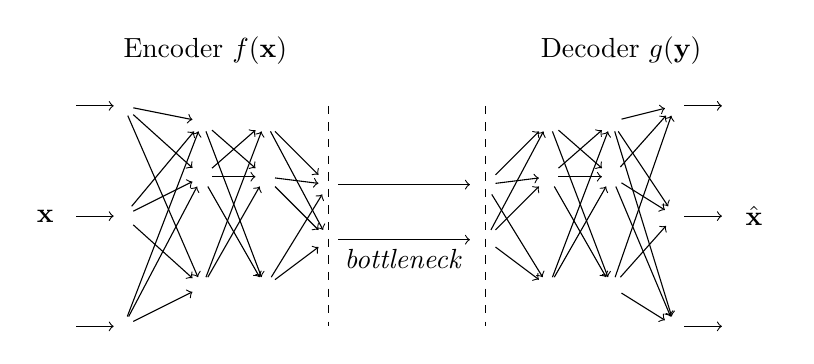
\begin{tikzpicture}
	%encoder
	\node[text width=3cm] at (1.5,2) {Encoder $f(\textbf{x})$};
	
	
	\draw [dashed] (2.6,1.3) -- (2.6,-1.5);
	
	\foreach \m [count=\y] in {1,missing,3,missing,5}
	\node [neuron/.try, neuron \m/.try] (input1-\m) at (0,2-\y*0.7) {};
	
	\foreach \m [count=\y] in {1,2,missing,4}
	\node [neuron/.try, neuron \m/.try ] (hidden1-\m) at (1,1.8-\y*0.7) {};
	
	\foreach \m [count=\y] in {1,2,missing,4}
	\node [neuron/.try, neuron \m/.try ] (hidden2-\m) at (1.8,1.8-\y*0.7) {};
	
	\foreach \m [count=\y] in {1,2}
	\node [neuron/.try, neuron \m/.try ] (output1-\m) at (2.6,1-\y*0.7) {};
	
	\node[text width=0.2cm] at (-1,-0.1) {$\textbf{x}$};
	
	
	\foreach \i in {1,3}
	\draw [<-] (input1-\i) -- ++(-0.6,0);
	
	\draw [->] (output1-1) -- ++(1.8,0);
	\draw [->] (output1-2) -- ++(1.8,0)
	node [below, midway] {\textit{bottleneck}};
	
	
	\draw [<-] (input1-5) -- ++(-0.6,0);

	%mesh1
	\foreach \i in {1,3,5} 
	\foreach \j in {1,2,4}
	\draw [->] (input1-\i) -- (hidden1-\j);
	
	\foreach \i in {1,2,4}
	\foreach \j in {2}
	\draw [->] (hidden1-\i) -- (hidden2-\j);
	
	\draw [->] (hidden1-2) -- (hidden2-1); 
	\draw [->] (hidden1-4) -- (hidden2-1); 
	
	\draw [->] (hidden1-1) -- (hidden2-4); 
	\draw [->] (hidden1-2) -- (hidden2-4); 
	
	\foreach \i in {1,2,4}
	\foreach \j in {1,2}
	\draw [->] (hidden2-\i) -- (output1-\j);
	
	\draw [dashed] (4.6,1.3) -- (4.6,-1.5);
	
	%decoder
	\node[text width=3cm] at (6.8,2) {Decoder $g(\textbf{y})$};
	\foreach \m [count=\y] in {1,2}
	\node [neuron/.try, neuron \m/.try ] (input2-\m) at (4.6,1-\y*0.7) {};
	
	\foreach \m [count=\y] in {1,2,missing,4}
	\node [neuron/.try, neuron \m/.try ] (hidden3-\m) at (5.4,1.8-\y*0.7) {};
	
	\foreach \m [count=\y] in {1,2,missing,4}
	\node [neuron/.try, neuron \m/.try ] (hidden4-\m) at (6.2,1.8-\y*0.7) {};
	
	\foreach \m [count=\y] in {1,missing,3,missing,5}
	\node [neuron/.try, neuron \m/.try] (output2-\m) at (7,2-\y*0.7) {};
	
	%outputs
	\foreach \i in {1,3,5}
	\draw [->] (output2-\i) -- ++(0.6,0);
	
	%mesh2
	\foreach \i in {1,2} 
	\foreach \j in {1,2,4}
	\draw [->] (input2-\i) -- (hidden3-\j);
	
	\foreach \i in {1,2,4}
	\foreach \j in {2}
	\draw [->] (hidden3-\i) -- (hidden4-\j);
	
	\draw [->] (hidden3-2) -- (hidden4-1); 
	\draw [->] (hidden3-4) -- (hidden4-1); 
	
	\draw [->] (hidden3-1) -- (hidden4-4); 
	\draw [->] (hidden3-2) -- (hidden4-4); 
	
	\foreach \i in {1,2,4}
	\foreach \j in {1,3,5}
	\draw [->] (hidden4-\i) -- (output2-\j);
	
	\node[text width=0.2cm] at (8,-0.1) {$\hat{\textbf{x}}$};
	
	
	
	
\end{tikzpicture}
}
\caption{Representation of the NN of an autoencoder.}
\label{fig:autoencoder}
\end{figure}

\end{frame}

\begin{frame}{Challenges}
	\begin{figure}
    \centering
	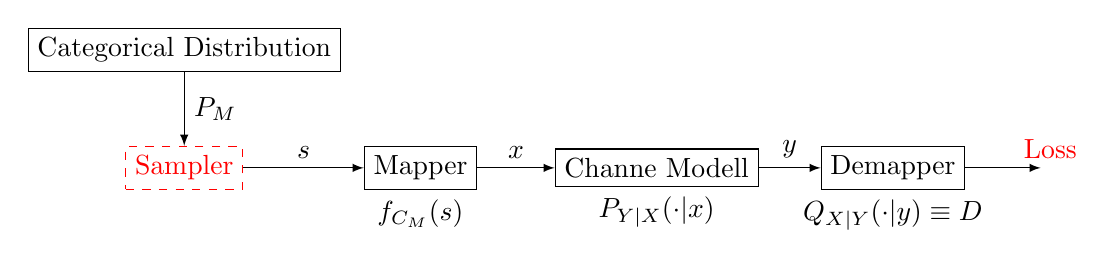
\begin{tikzpicture}
		\node[draw] at (0,1.5) (dist){Categorical Distribution};
		\node[draw, style=dashed, color=red] at (0,0) (sampler){Sampler};
		\node[draw, label=below:$f_{C_M}(s)$]  at (3,0) (map){Mapper};
		\node[draw, label=below:$P_{Y|X}(\cdot|x)$] at (6,0) (ch) {Channe Modell};
		\node[draw, label=below:$Q_{X|Y}(\cdot|y) \equiv D$] at (9,0) (demap) {Demapper};
		\node(dst) at (11,0){};
		
		\draw[-latex] (dist) --  (sampler) node[midway,right] {$P_M$};	
		\draw[-latex] (sampler) --  (map) node[midway,above] {$s$};		
		\draw[-latex] (map) --  (ch) node[midway,above] {$x$};
		\draw[-latex] (ch) -- (demap) node[midway,above] {$y$};	
		\draw[-latex] (demap) --(dst) node[right, above, color=red]{Loss};

	\end{tikzpicture}
	\end{figure}
	\vspace{-5mm}
	\begin{itemize}
	\item To find fitting sets of parameters $\{P_M, C_M, D\}$ we define a loss function,  $L(P_M, C_M, D)$, that compares the current output of the autoencoder with the desired output from the training set.
	\item The most used algorithm is SGD, which trains any parameter, $\theta$, as
	\begin{align*}
	{\theta}_{new} = {\theta}_{old} + \epsilon \grad L({\theta}_{old}) %, \qquad \boldsymbol{\theta} \in \{\bold{W_k}, \bold{b_k}\}
	\end{align*}
	\item To compute the gradient efficiently a computational graph stores the transformations to the factors which influenced the loss function. %Automatic differentiation (pytorch cannot handle complex numbers)
	\end{itemize}
\end{frame}



\begin{frame}{First implementation \cite{Stark}}
	Trainable parameters:
	\vspace{-5mm}
	\begin{itemize}
		\item $P_M$, source's probability distribution learnt by the encoder.
		\item $C_M$, spatial distribution of the constellation points learnt by the mapper.
		\item $D$, posterior probability distribution learnt by the demapper.
	\end{itemize}
	\vspace{-5mm}
	Autoencoder architecture:
	\begin{figure}
		\centering
		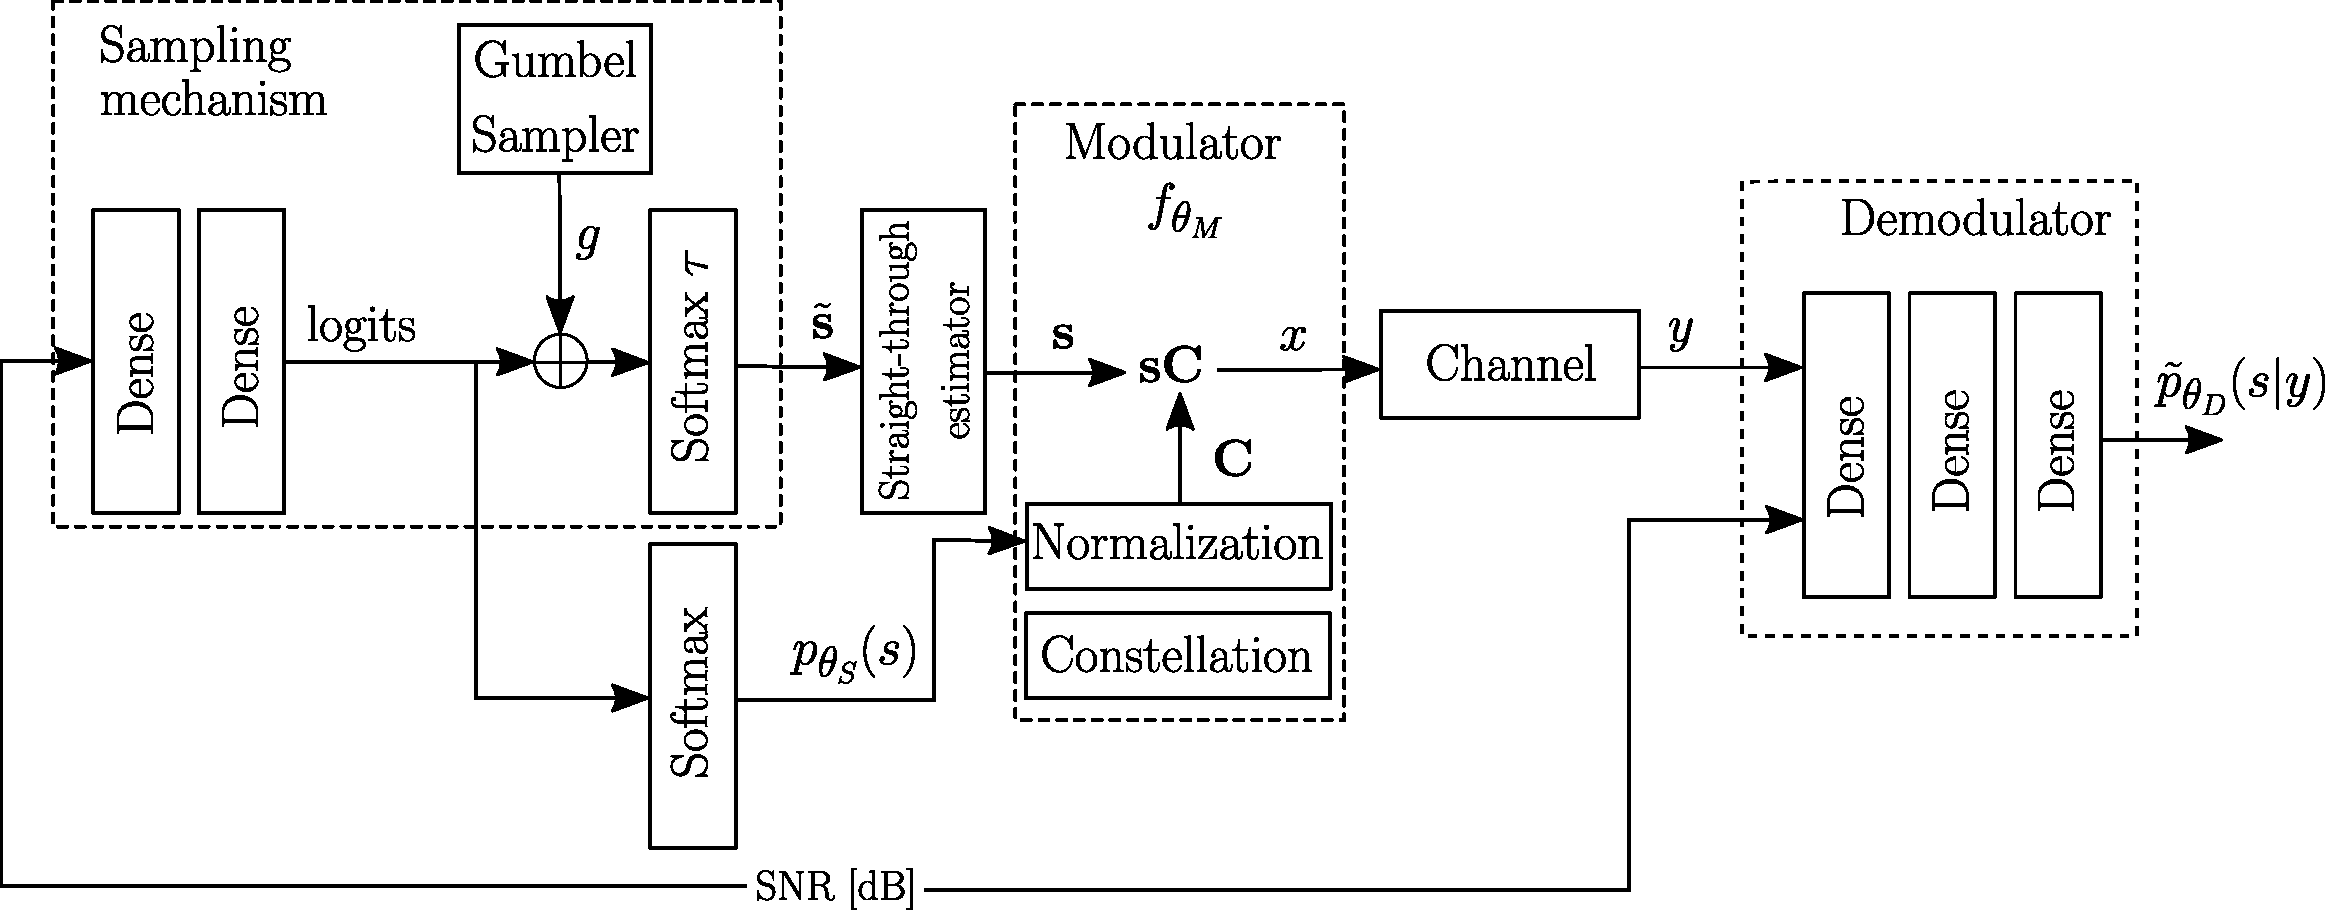
\includegraphics[width=0.6\columnwidth]{stark_diagram.pdf}
%		\caption{Proposed Autoencoder Architecture from \cite{Stark}}
		\label{fig:starkAe}
	\end{figure}
\end{frame}

\begin{frame}{Loss Function}
	The goal of probabilistic constellation shaping is to maximize the MI. To this end, defining an appropriate loss function is critical. Starting from the demodulator, the categorical cross entropy loss
\begin{align*}
	L(D, P_M, C_M) \triangleq \mathbb{X}(P_{X|Y}||Q_{X|Y}; D) = \mathbb{E}\left[-\log_2(Q(X|Y;D))\right] 
\end{align*}
is appropriate for training $D$ and $C_M$, but not $P_M$. To see why, we rewrite the MI as
\begin{align*}
	\mathbb{I} \left(X , Y\right) &= \mathbb{H}(X) - \mathbb{H}(X|Y)\\
	\mathbb{I} \left(X , Y\right) &= \mathbb{H}(X) - \mathbb{X}(P_{X|Y}||Q_{X|Y}) + \mathbb{D}(P_{X|Y}||Q_{X|Y}).
\end{align*}
And the Loss becomes
\begin{align*}
L(D, P_M, C_M) &= \mathbb{H}(X) -\mathbb{I} \left(X , Y\right) + \mathbb{D}(P_{X|Y}||Q_{X|Y}).
\end{align*}
So, if $L$ is minimized during training, the source entropy is unwantedly minimized.
%If we minimize the cross entropy loss we would also minimize the source entropy. A modification of this loss function is necessary.
\end{frame}

\begin{frame}{Loss Function (cont'd)}
To avoid this effect, \citeauthor{Stark} modify the loss function as
\begin{align*}
	\hat{L}(D, P_M, C_M) \triangleq L(D, P_M, C_M) - \mathbb{H}(X).
\end{align*}
With this correction the optimization problem 
\begin{align*}
	\min_{D, P_M, C_M}\hat{L}(D, P_M, C_M) = \max_{D, P_M, C_M} \{ \mathbb{I} \left(X , Y\right) - \mathbb{D}(P_{X|Y}||Q_{X|Y})\}
\end{align*}
maximizes the MI.
\end{frame}

\begin{frame}{Gumbel-Softmax trick \cite{JANG}}
\begin{itemize}
\item Solves the problem of backpropagating through stochastic nodes by reparametrizing the samples to avoid breaking the dependency between the samples and the trainable parameters.
\item Relaxes the argmax function using a softmax instead, which is smooth in $\tau > 0$. The parameter $\tau$, controls the degree of approximation to the expected value of the categorical distribution.
\end{itemize}
\begin{figure}
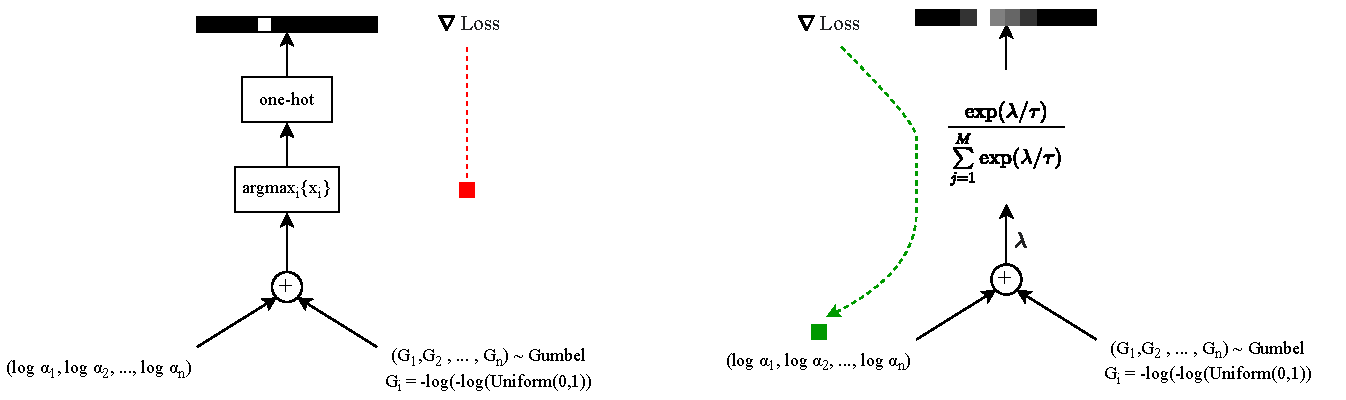
\includegraphics[width=0.85\columnwidth]{ressources/Gumbel_Softmax.pdf}
\caption{ Non-differentiable path vs. differentiable path using the Gumbel-Softmax trick. }
\end{figure}
\end{frame}

\begin{frame}{Probabilistic Constellation Shaping}
\begin{figure}
	\subfigure[5dB]{
		\input{../documentation/figs/stark_pcs_5db}
		\label{subfig:stark_pcs_5db}
	}
	\subfigure[18db]{
		\input{../documentation/figs/stark_pcs_18db}
		\label{subfig:stark_pcs_18db}
	}
	\caption{Learnt probabilistic constellation shaping for M = 64. The size of the markers is proportional to the transmission probability of the symbol. When trained under 5dB, the probabilistic shaping approaches a Gaussian. While under 18dB it approaches a uniform distribution. }
\end{figure}
\end{frame}

\begin{frame}{Joint Probabilistic and Geometric Shaping}
\begin{figure}[h]
	\subfigure[SNR = 5dB]{
         \input{../documentation/figs/stark_gcs_5db}
         \label{subfig:stark5dB}
    }
    \subfigure[SNR = 18dB]{
         \input{../documentation/figs/stark_gcs_18db}
         \label{subfig:stark18dB}
    }
    \caption{Learnt joint geometric and probabilistic ASK constellations for M=8.}
    \label{fig:starkMASK}
\end{figure}

\end{frame}

\begin{frame}{Overall Performance}
\begin{figure}[H]
	\centering
	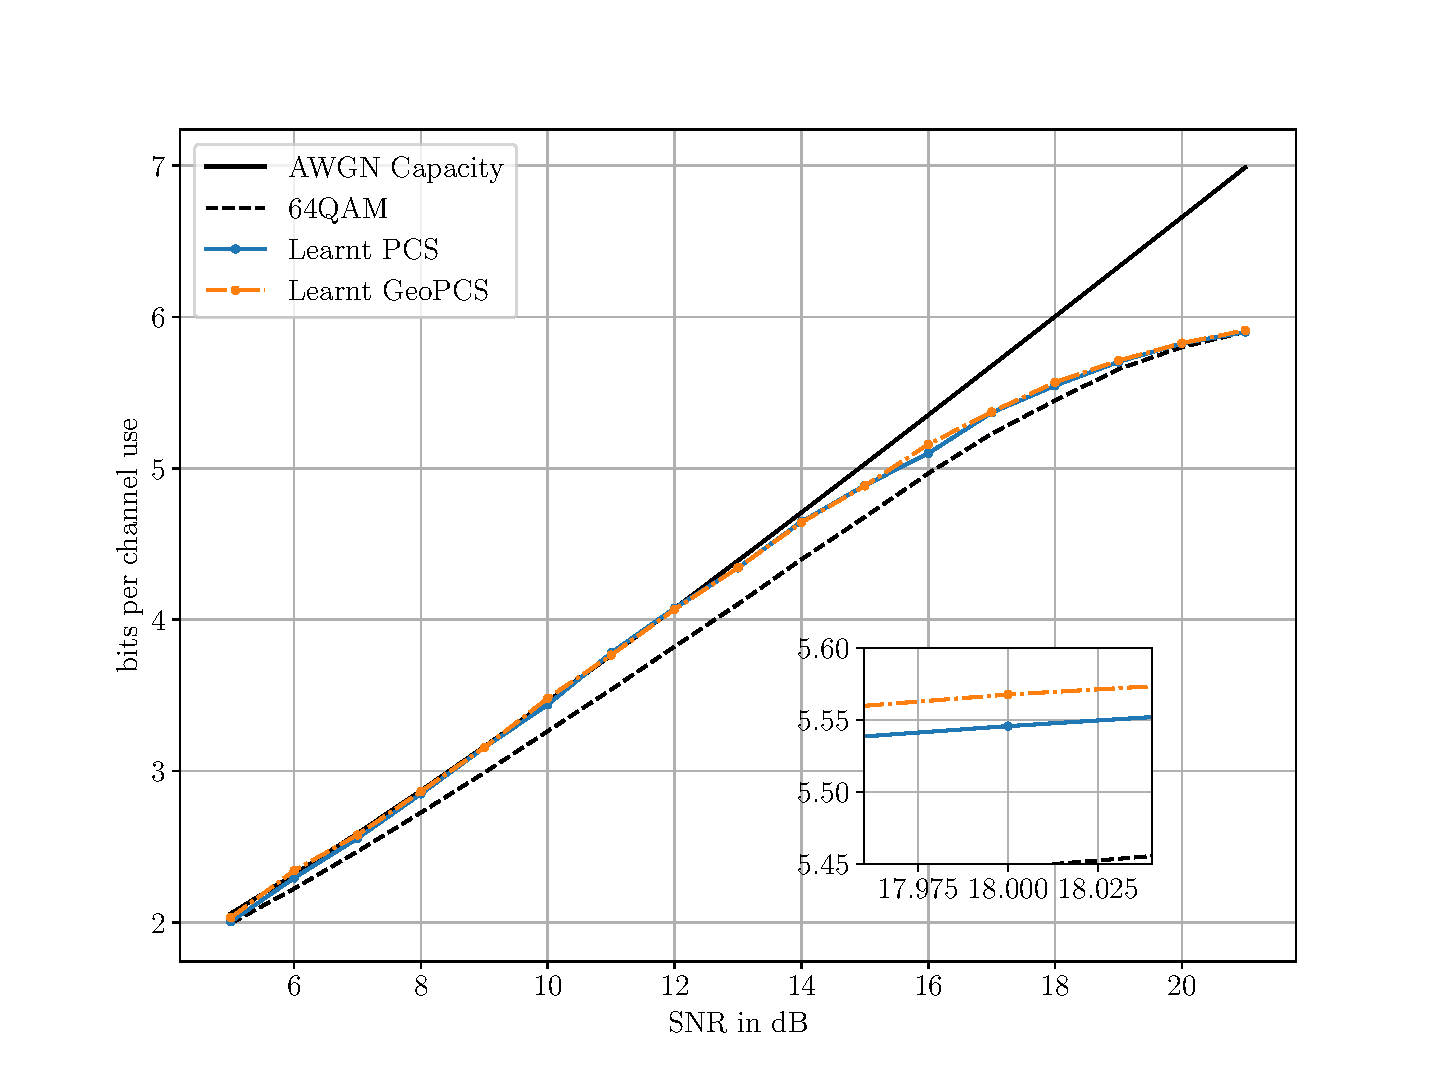
\includegraphics[width=0.75\columnwidth]{stark_gcs.pdf}
%    \caption{Mutual information learned by the PCS and GeoPCS for constellation size M=64 on the AWGN channel. Zoom is for the 18dB point.}
    \label{fig:starkPerf}
\end{figure}
\end{frame}

\begin{frame}{Second implementation \cite{Aref}}
	What motivates another implementation?\\
	\textit{The Gumbel-Softmax trick is complex and numerically unstable.\\}
	Trainable parameters:
	\vspace{-5mm}
	\begin{itemize}
		\item $P_M$, source's probability distribution learnt by the sampler.
		\item $C_M$, spatial distribution of the constellation points learnt by the mapper.
		\item $D$, posterior probability distribution learnt by the demapper.
	\end{itemize}
	
    \begin{figure}
		\centering
		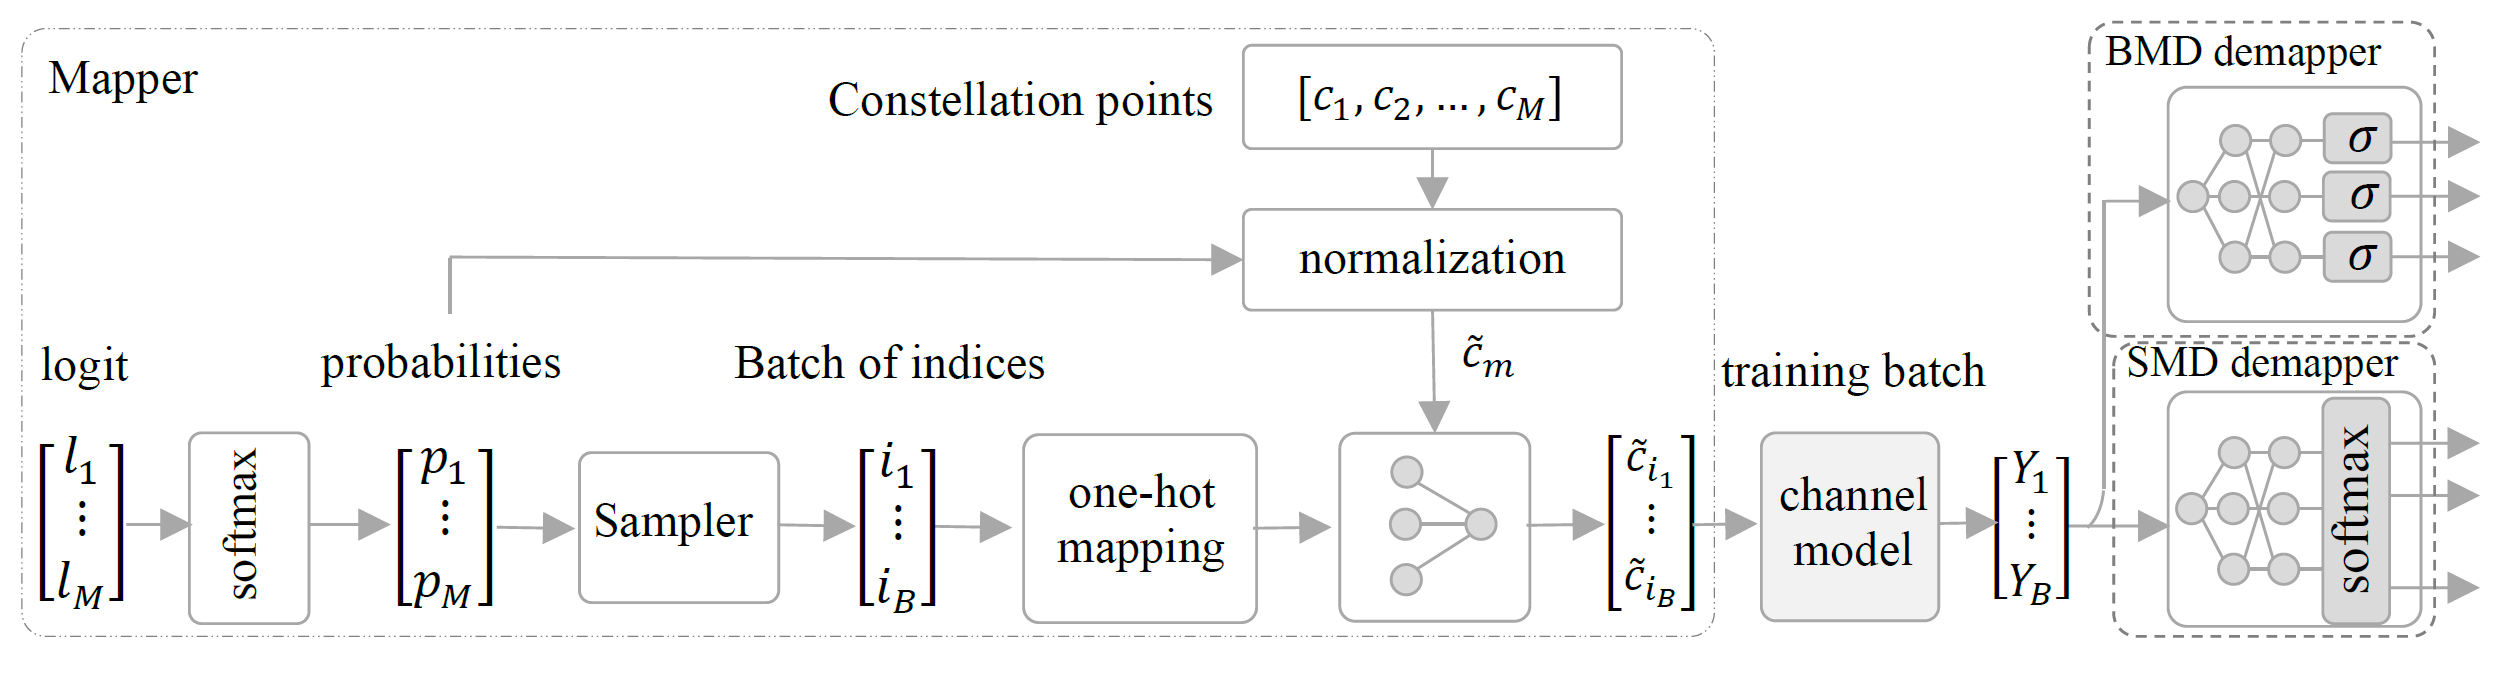
\includegraphics[width=0.8\columnwidth]{aref_diagram.png}
	%	\caption{Proposed Autoencoder Architecture from \cite{Aref}}
		\label{fig:arefAe}
	\end{figure}
\end{frame}

\begin{frame}{Loss Function}
	The goal is again to to maximize the mutual information
	\begin{align}
		 \max_{D, P_M, C_M} \mathbb{I} \left(X , Y ; D, P_M, C_M \right) = \mathbb{H}(X) - \mathbb{X}(P_{X|Y} \Vert Q_{X|Y} ; D, P_M, C_M).
	\end{align}
	
	Typically, through SGD we adjust the trainable parameters as:
	\begin{align}
		\theta_{new} = \theta_{old} + \epsilon \pdv{\theta_{old}} \mathbb{I} \left(X , Y ; \theta_{old} \right)
	\end{align}
	for all trainable parameters $\theta \in P_M, C_M, D$. And the MI can be numerically approximated by
	\begin{align}
		\mathbb{I} \left(X , Y\right) \approx \mathbb{I} \left(X , Y\right)_{\text{num}} &= \dfrac{1}{B} \sum \limits_{i = 1}^{B} - \log_2(P(x_i)) + \log_2(Q_{X|Y}(x_i|y_i))\\
		&= \dfrac{1}{B} \sum \limits_{i = 1}^{B} L(x_i, y_i).
	\end{align}
\end{frame}

\begin{frame}
	Next, the following approximation usually allows to adjust the trainable parameters:
	\begin{align}
		\pdv{\theta} \mathbb{I} \left(X , Y ; \theta \right) \approx \pdv{\theta} \mathbb{I} \left(X , Y\right)_{\text{num}} = \dfrac{1}{B} \sum \limits_{i = 1}^{B} L(x_i, y_i).
	\end{align}
	
	However, Aref claims that although this is true for the constellation locations $(\theta \in C_M)$ and the demapper parameters $(\theta \in D)$, it does not hold for the constellation probabilities $\{p_1, p_2, \dots, p_M\} = P_M$
	\begin{align}
	\label{eqn:mi_pdv_p}
		\pdv{p_j} \mathbb{I} \left(X , Y ; P_M \right) \not\approx \dfrac{1}{B} \sum \limits_{i = 1}^{B} \pdv{p_j} L(x_i, y_i)
	\end{align}
	
	as $\{p_1, p_2, \dots, p_M\}$ changes the statistics of the training set.
	
	For this reason, (\ref{eqn:mi_pdv_p}) must be computed differently.
	
	\end{frame}

\begin{frame}
\begin{itemize}
	\item Instead of relying on the autodifferentiation mechanism, \citeauthor{Aref} compute the gradient analytically.\\
 	\item The derivative of the mutual information w.r.t. $p_j$, (\ref{eqn:mi_pdv_p}), results to be
	\begin{align}
		\pdv{p_j} \mathbb{I} \left(X , Y ; P_M \right) \approx - \log_2 (p_j) - \log_2 (e) + \dfrac{1}{Bp_j}\sum \limits_{b \text{ if } x=j} \log_2 Q_{X|Y}(j|b) + \dfrac{1}{B} \sum \limits_{(a,b)} \log_2 Q_{X|Y}(a|b)
	\end{align}
	
	\item The following terms can be computed via backpropagation
	\begin{align}
		- \log_2 (p_j) + \dfrac{1}{Bp_j}\sum \limits_{b \text{ if } x=j} \log_2 Q_{X|Y}(j|b) = \dfrac{1}{B} \sum \limits_{i = 1}^{B} \pdv{p_j} L(x_i, y_i)
	\end{align}
	while the remaining ones must be explicitly computed and added to the gradient after backpropagating.
	\item We call this step \textit{gradient correction} and it is due to the change of statistics in the sampled batch.
\end{itemize}
\end{frame}
	

\begin{frame}{Probabilistic Shaping}
	\begin{figure}
\centering
\subfigure[SNR = 5dB]{
	% This file was created with tikzplotlib v0.10.1.
	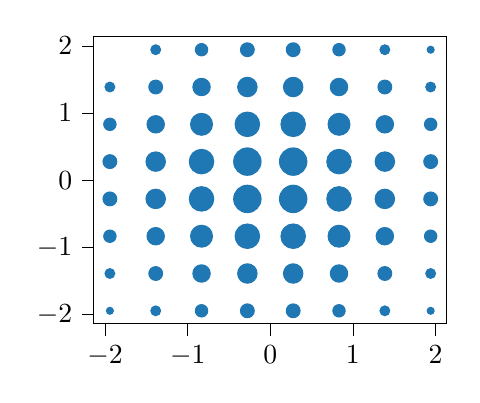
\begin{tikzpicture}
	
	\definecolor{darkgray176}{RGB}{176,176,176}
	\definecolor{steelblue31119180}{RGB}{31,119,180}
	
	\begin{axis}[
	width=0.5\columnwidth,
	tick align=outside,
	tick pos=left,
	x grid style={darkgray176},
	xmin=-2.13620593547821, xmax=2.13620593547821,
	xtick style={color=black},
	y grid style={darkgray176},
	ymin=-2.13620593547821, ymax=2.13620593547821,
	ytick style={color=black}
	]
	\addplot [
	  mark=*,
	  only marks,
	  scatter,
	  scatter/use mapped color={
	    draw=steelblue31119180,
	    fill=steelblue31119180,
	  },
	  scatter/@pre marker code/.append style={/tikz/mark size=\perpointmarksize},
	  visualization depends on={\thisrow{sizedata} \as\perpointmarksize},
	  table/row sep=\\
	]
	table{%
	x  y  sizedata
	-1.94200539588928 1.94200539588928 1.2521708\\
	-1.38714671134949 1.94200539588928 1.7632555\\
	-0.832288026809692 1.94200539588928 2.2239556\\
	-0.277429342269897 1.94200539588928 2.4847505\\
	0.277429342269897 1.94200539588928 2.4847505\\
	0.832288026809692 1.94200539588928 2.2239556\\
	1.38714671134949 1.94200539588928 1.7632555\\
	1.94200539588928 1.94200539588928 1.2521708\\
	-1.94200539588928 1.38714671134949 1.7632555\\
	-1.38714671134949 1.38714671134949 2.4829438\\
	-0.832288026809692 1.38714671134949 3.1316829\\
	-0.277429342269897 1.38714671134949 3.4989233\\
	0.277429342269897 1.38714671134949 3.4989233\\
	0.832288026809692 1.38714671134949 3.1316829\\
	1.38714671134949 1.38714671134949 2.4829438\\
	1.94200539588928 1.38714671134949 1.7632555\\
	-1.94200539588928 0.832288026809692 2.2239556\\
	-1.38714671134949 0.832288026809692 3.1316829\\
	-0.832288026809692 0.832288026809692 3.9499235\\
	-0.277429342269897 0.832288026809692 4.413116\\
	0.277429342269897 0.832288026809692 4.413116\\
	0.832288026809692 0.832288026809692 3.9499235\\
	1.38714671134949 0.832288026809692 3.1316829\\
	1.94200539588928 0.832288026809692 2.2239556\\
	-1.94200539588928 0.277429342269897 2.4847505\\
	-1.38714671134949 0.277429342269897 3.4989233\\
	-0.832288026809692 0.277429342269897 4.413116\\
	-0.277429342269897 0.277429342269897 4.9306254\\
	0.277429342269897 0.277429342269897 4.9306254\\
	0.832288026809692 0.277429342269897 4.413116\\
	1.38714671134949 0.277429342269897 3.4989233\\
	1.94200539588928 0.277429342269897 2.4847505\\
	-1.94200539588928 -0.277429342269897 2.4847505\\
	-1.38714671134949 -0.277429342269897 3.4989233\\
	-0.832288026809692 -0.277429342269897 4.413116\\
	-0.277429342269897 -0.277429342269897 4.9306254\\
	0.277429342269897 -0.277429342269897 4.9306254\\
	0.832288026809692 -0.277429342269897 4.413116\\
	1.38714671134949 -0.277429342269897 3.4989233\\
	1.94200539588928 -0.277429342269897 2.4847505\\
	-1.94200539588928 -0.832288026809692 2.2239556\\
	-1.38714671134949 -0.832288026809692 3.1316829\\
	-0.832288026809692 -0.832288026809692 3.9499235\\
	-0.277429342269897 -0.832288026809692 4.413116\\
	0.277429342269897 -0.832288026809692 4.413116\\
	0.832288026809692 -0.832288026809692 3.9499235\\
	1.38714671134949 -0.832288026809692 3.1316829\\
	1.94200539588928 -0.832288026809692 2.2239556\\
	-1.94200539588928 -1.38714671134949 1.7632555\\
	-1.38714671134949 -1.38714671134949 2.4829438\\
	-0.832288026809692 -1.38714671134949 3.1316829\\
	-0.277429342269897 -1.38714671134949 3.4989233\\
	0.277429342269897 -1.38714671134949 3.4989233\\
	0.832288026809692 -1.38714671134949 3.1316829\\
	1.38714671134949 -1.38714671134949 2.4829438\\
	1.94200539588928 -1.38714671134949 1.7632555\\
	-1.94200539588928 -1.94200539588928 1.2521708\\
	-1.38714671134949 -1.94200539588928 1.7632555\\
	-0.832288026809692 -1.94200539588928 2.2239556\\
	-0.277429342269897 -1.94200539588928 2.4847505\\
	0.277429342269897 -1.94200539588928 2.4847505\\
	0.832288026809692 -1.94200539588928 2.2239556\\
	1.38714671134949 -1.94200539588928 1.7632555\\
	1.94200539588928 -1.94200539588928 1.2521708\\
	};
	\end{axis}
	
	\end{tikzpicture}
}
\subfigure[SNR = 18dB]{
	% This file was created with tikzplotlib v0.10.1.
	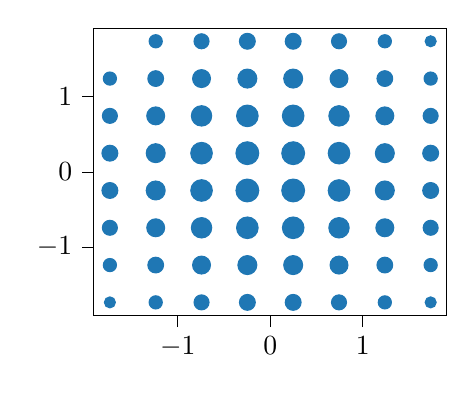
\begin{tikzpicture}
	
	\definecolor{darkgray176}{RGB}{176,176,176}
	\definecolor{steelblue31119180}{RGB}{31,119,180}
	
	\begin{axis}[
	width=0.5\columnwidth,
	tick align=outside,
	tick pos=left,
	x grid style={darkgray176},
	xmin=-1.90730187892914, xmax=1.90730187892914,
	xtick style={color=black},
	y grid style={darkgray176},
	ymin=-1.90730187892914, ymax=1.90730187892914,
	ytick style={color=black}
	]
	\addplot [
	  mark=*,
	  only marks,
	  scatter,
	  scatter/use mapped color={
	    draw=steelblue31119180,
	    fill=steelblue31119180,
	  },
	  scatter/@pre marker code/.append style={/tikz/mark size=\perpointmarksize},
	  visualization depends on={\thisrow{sizedata} \as\perpointmarksize},
	  table/row sep=\\
	]
	table{%
	x  y  sizedata
	-1.73391079902649 1.73391079902649 1.9902518\\
	-1.23850774765015 1.73391079902649 2.3760042\\
	-0.743104636669159 1.73391079902649 2.7039983\\
	-0.247701555490494 1.73391079902649 2.8618598\\
	0.247701555490494 1.73391079902649 2.8618598\\
	0.743104636669159 1.73391079902649 2.7039983\\
	1.23850774765015 1.73391079902649 2.3760042\\
	1.73391079902649 1.73391079902649 1.9902518\\
	-1.73391079902649 1.23850774765015 2.3760042\\
	-1.23850774765015 1.23850774765015 2.8365235\\
	-0.743104636669159 1.23850774765015 3.2280898\\
	-0.247701555490494 1.23850774765015 3.416548\\
	0.247701555490494 1.23850774765015 3.416548\\
	0.743104636669159 1.23850774765015 3.2280898\\
	1.23850774765015 1.23850774765015 2.8365235\\
	1.73391079902649 1.23850774765015 2.3760042\\
	-1.73391079902649 0.743104636669159 2.7039983\\
	-1.23850774765015 0.743104636669159 3.2280898\\
	-0.743104636669159 0.743104636669159 3.6737092\\
	-0.247701555490494 0.743104636669159 3.8881829\\
	0.247701555490494 0.743104636669159 3.8881829\\
	0.743104636669159 0.743104636669159 3.6737092\\
	1.23850774765015 0.743104636669159 3.2280898\\
	1.73391079902649 0.743104636669159 2.7039983\\
	-1.73391079902649 0.247701555490494 2.8618598\\
	-1.23850774765015 0.247701555490494 3.416548\\
	-0.743104636669159 0.247701555490494 3.8881829\\
	-0.247701555490494 0.247701555490494 4.115178\\
	0.247701555490494 0.247701555490494 4.115178\\
	0.743104636669159 0.247701555490494 3.8881829\\
	1.23850774765015 0.247701555490494 3.416548\\
	1.73391079902649 0.247701555490494 2.8618598\\
	-1.73391079902649 -0.247701555490494 2.8618598\\
	-1.23850774765015 -0.247701555490494 3.416548\\
	-0.743104636669159 -0.247701555490494 3.8881829\\
	-0.247701555490494 -0.247701555490494 4.115178\\
	0.247701555490494 -0.247701555490494 4.115178\\
	0.743104636669159 -0.247701555490494 3.8881829\\
	1.23850774765015 -0.247701555490494 3.416548\\
	1.73391079902649 -0.247701555490494 2.8618598\\
	-1.73391079902649 -0.743104636669159 2.7039983\\
	-1.23850774765015 -0.743104636669159 3.2280898\\
	-0.743104636669159 -0.743104636669159 3.6737092\\
	-0.247701555490494 -0.743104636669159 3.8881829\\
	0.247701555490494 -0.743104636669159 3.8881829\\
	0.743104636669159 -0.743104636669159 3.6737092\\
	1.23850774765015 -0.743104636669159 3.2280898\\
	1.73391079902649 -0.743104636669159 2.7039983\\
	-1.73391079902649 -1.23850774765015 2.3760042\\
	-1.23850774765015 -1.23850774765015 2.8365235\\
	-0.743104636669159 -1.23850774765015 3.2280898\\
	-0.247701555490494 -1.23850774765015 3.416548\\
	0.247701555490494 -1.23850774765015 3.416548\\
	0.743104636669159 -1.23850774765015 3.2280898\\
	1.23850774765015 -1.23850774765015 2.8365235\\
	1.73391079902649 -1.23850774765015 2.3760042\\
	-1.73391079902649 -1.73391079902649 1.9902518\\
	-1.23850774765015 -1.73391079902649 2.3760042\\
	-0.743104636669159 -1.73391079902649 2.7039983\\
	-0.247701555490494 -1.73391079902649 2.8618598\\
	0.247701555490494 -1.73391079902649 2.8618598\\
	0.743104636669159 -1.73391079902649 2.7039983\\
	1.23850774765015 -1.73391079902649 2.3760042\\
	1.73391079902649 -1.73391079902649 1.9902518\\
	};
	\end{axis}
	
	\end{tikzpicture}
}
\caption{Learnt probabilistic constellation shaping for M = 64. The size of the markers is proportional to the transmission probability of the symbol. When trained under 5dB, the proababilistic shaping approaches a gaussian. While under 18dB it approaches a uniform distribution. }
\end{figure}


\end{frame}

\begin{frame}{Joint Geometric and Probabilistic Shaping}
	\begin{figure}

\subfigure[SNR = 5dB]{
	% This file was created with tikzplotlib v0.10.1.
	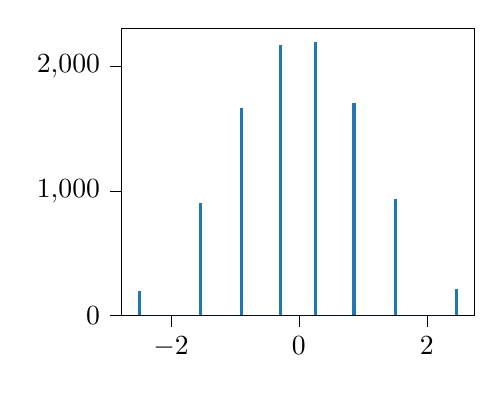
\begin{tikzpicture}
	
	\definecolor{darkgray176}{RGB}{176,176,176}
	\definecolor{steelblue31119180}{RGB}{31,119,180}
	
	\begin{axis}[
	width=0.5\columnwidth,
	tick align=outside,
	tick pos=left,
	x grid style={darkgray176},
	xmin=-2.77227712869644, xmax=2.74234153032303,
	xtick style={color=black},
	y grid style={darkgray176},
	ymin=0, ymax=2307.9,
	ytick style={color=black}
	]
	\draw[draw=none,fill=steelblue31119180] (axis cs:-2.52161264419556,0) rectangle (axis cs:-2.47147965431213,199);
	\draw[draw=none,fill=steelblue31119180] (axis cs:-2.47147965431213,0) rectangle (axis cs:-2.42134690284729,0);
	\draw[draw=none,fill=steelblue31119180] (axis cs:-2.42134666442871,0) rectangle (axis cs:-2.37121367454529,0);
	\draw[draw=none,fill=steelblue31119180] (axis cs:-2.37121391296387,0) rectangle (axis cs:-2.32108116149902,0);
	\draw[draw=none,fill=steelblue31119180] (axis cs:-2.32108116149902,0) rectangle (axis cs:-2.2709481716156,0);
	\draw[draw=none,fill=steelblue31119180] (axis cs:-2.27094793319702,0) rectangle (axis cs:-2.2208149433136,0);
	\draw[draw=none,fill=steelblue31119180] (axis cs:-2.22081518173218,0) rectangle (axis cs:-2.17068243026733,0);
	\draw[draw=none,fill=steelblue31119180] (axis cs:-2.17068243026733,0) rectangle (axis cs:-2.12054944038391,0);
	\draw[draw=none,fill=steelblue31119180] (axis cs:-2.12054944038391,0) rectangle (axis cs:-2.07041668891907,0);
	\draw[draw=none,fill=steelblue31119180] (axis cs:-2.07041645050049,0) rectangle (axis cs:-2.02028346061707,0);
	\draw[draw=none,fill=steelblue31119180] (axis cs:-2.02028369903564,0) rectangle (axis cs:-1.9701509475708,0);
	\draw[draw=none,fill=steelblue31119180] (axis cs:-1.97015070915222,0) rectangle (axis cs:-1.92001795768738,0);
	\draw[draw=none,fill=steelblue31119180] (axis cs:-1.92001795768738,0) rectangle (axis cs:-1.86988496780396,0);
	\draw[draw=none,fill=steelblue31119180] (axis cs:-1.86988496780396,0) rectangle (axis cs:-1.81975221633911,0);
	\draw[draw=none,fill=steelblue31119180] (axis cs:-1.81975197792053,0) rectangle (axis cs:-1.76961922645569,0);
	\draw[draw=none,fill=steelblue31119180] (axis cs:-1.76961922645569,0) rectangle (axis cs:-1.71948647499084,0);
	\draw[draw=none,fill=steelblue31119180] (axis cs:-1.71948623657227,0) rectangle (axis cs:-1.66935348510742,0);
	\draw[draw=none,fill=steelblue31119180] (axis cs:-1.66935348510742,0) rectangle (axis cs:-1.619220495224,0);
	\draw[draw=none,fill=steelblue31119180] (axis cs:-1.619220495224,0) rectangle (axis cs:-1.56908774375916,0);
	\draw[draw=none,fill=steelblue31119180] (axis cs:-1.56908750534058,0) rectangle (axis cs:-1.51895475387573,905);
	\draw[draw=none,fill=steelblue31119180] (axis cs:-1.51895475387573,0) rectangle (axis cs:-1.46882200241089,0);
	\draw[draw=none,fill=steelblue31119180] (axis cs:-1.46882176399231,0) rectangle (axis cs:-1.41868901252747,0);
	\draw[draw=none,fill=steelblue31119180] (axis cs:-1.41868901252747,0) rectangle (axis cs:-1.36855602264404,0);
	\draw[draw=none,fill=steelblue31119180] (axis cs:-1.36855602264404,0) rectangle (axis cs:-1.3184232711792,0);
	\draw[draw=none,fill=steelblue31119180] (axis cs:-1.31842303276062,0) rectangle (axis cs:-1.26829028129578,0);
	\draw[draw=none,fill=steelblue31119180] (axis cs:-1.26829028129578,0) rectangle (axis cs:-1.21815752983093,0);
	\draw[draw=none,fill=steelblue31119180] (axis cs:-1.21815729141235,0) rectangle (axis cs:-1.16802453994751,0);
	\draw[draw=none,fill=steelblue31119180] (axis cs:-1.16802453994751,0) rectangle (axis cs:-1.11789155006409,0);
	\draw[draw=none,fill=steelblue31119180] (axis cs:-1.11789155006409,0) rectangle (axis cs:-1.06775879859924,0);
	\draw[draw=none,fill=steelblue31119180] (axis cs:-1.06775856018066,0) rectangle (axis cs:-1.01762580871582,0);
	\draw[draw=none,fill=steelblue31119180] (axis cs:-1.01762580871582,0) rectangle (axis cs:-0.967493057250977,0);
	\draw[draw=none,fill=steelblue31119180] (axis cs:-0.967492938041687,0) rectangle (axis cs:-0.917359948158264,0);
	\draw[draw=none,fill=steelblue31119180] (axis cs:-0.917359948158264,0) rectangle (axis cs:-0.86722719669342,1663);
	\draw[draw=none,fill=steelblue31119180] (axis cs:-0.86722719669342,0) rectangle (axis cs:-0.817094206809998,0);
	\draw[draw=none,fill=steelblue31119180] (axis cs:-0.817094147205353,0) rectangle (axis cs:-0.766961395740509,0);
	\draw[draw=none,fill=steelblue31119180] (axis cs:-0.766961276531219,0) rectangle (axis cs:-0.716828525066376,0);
	\draw[draw=none,fill=steelblue31119180] (axis cs:-0.716828465461731,0) rectangle (axis cs:-0.666695475578308,0);
	\draw[draw=none,fill=steelblue31119180] (axis cs:-0.666695475578308,0) rectangle (axis cs:-0.616562724113464,0);
	\draw[draw=none,fill=steelblue31119180] (axis cs:-0.616562724113464,0) rectangle (axis cs:-0.566429734230042,0);
	\draw[draw=none,fill=steelblue31119180] (axis cs:-0.566429674625397,0) rectangle (axis cs:-0.516296923160553,0);
	\draw[draw=none,fill=steelblue31119180] (axis cs:-0.516296923160553,0) rectangle (axis cs:-0.46616393327713,0);
	\draw[draw=none,fill=steelblue31119180] (axis cs:-0.466163992881775,0) rectangle (axis cs:-0.416031002998352,0);
	\draw[draw=none,fill=steelblue31119180] (axis cs:-0.416031002998352,0) rectangle (axis cs:-0.365898251533508,0);
	\draw[draw=none,fill=steelblue31119180] (axis cs:-0.365898251533508,0) rectangle (axis cs:-0.315765261650085,0);
	\draw[draw=none,fill=steelblue31119180] (axis cs:-0.31576532125473,0) rectangle (axis cs:-0.265632331371307,2174);
	\draw[draw=none,fill=steelblue31119180] (axis cs:-0.265632450580597,0) rectangle (axis cs:-0.215499460697174,0);
	\draw[draw=none,fill=steelblue31119180] (axis cs:-0.215499550104141,0) rectangle (axis cs:-0.165366560220718,0);
	\draw[draw=none,fill=steelblue31119180] (axis cs:-0.165366649627686,0) rectangle (axis cs:-0.115233659744263,0);
	\draw[draw=none,fill=steelblue31119180] (axis cs:-0.11523374915123,0) rectangle (axis cs:-0.065100759267807,0);
	\draw[draw=none,fill=steelblue31119180] (axis cs:-0.0651008635759354,0) rectangle (axis cs:-0.0149678736925125,0);
	\draw[draw=none,fill=steelblue31119180] (axis cs:-0.01496796682477,0) rectangle (axis cs:0.0351650230586529,0);
	\draw[draw=none,fill=steelblue31119180] (axis cs:0.0351649262011051,0) rectangle (axis cs:0.0852979123592377,0);
	\draw[draw=none,fill=steelblue31119180] (axis cs:0.0852978229522705,0) rectangle (axis cs:0.135430812835693,0);
	\draw[draw=none,fill=steelblue31119180] (axis cs:0.135430723428726,0) rectangle (axis cs:0.185563713312149,0);
	\draw[draw=none,fill=steelblue31119180] (axis cs:0.185563609004021,0) rectangle (axis cs:0.235696598887444,0);
	\draw[draw=none,fill=steelblue31119180] (axis cs:0.235696494579315,0) rectangle (axis cs:0.285829484462738,2198);
	\draw[draw=none,fill=steelblue31119180] (axis cs:0.285829424858093,0) rectangle (axis cs:0.335962414741516,0);
	\draw[draw=none,fill=steelblue31119180] (axis cs:0.335962414741516,0) rectangle (axis cs:0.38609516620636,0);
	\draw[draw=none,fill=steelblue31119180] (axis cs:0.38609516620636,0) rectangle (axis cs:0.436228156089783,0);
	\draw[draw=none,fill=steelblue31119180] (axis cs:0.436228096485138,0) rectangle (axis cs:0.486361086368561,0);
	\draw[draw=none,fill=steelblue31119180] (axis cs:0.486361086368561,0) rectangle (axis cs:0.536493837833405,0);
	\draw[draw=none,fill=steelblue31119180] (axis cs:0.536493897438049,0) rectangle (axis cs:0.586626887321472,0);
	\draw[draw=none,fill=steelblue31119180] (axis cs:0.586626887321472,0) rectangle (axis cs:0.636759638786316,0);
	\draw[draw=none,fill=steelblue31119180] (axis cs:0.636759638786316,0) rectangle (axis cs:0.686892628669739,0);
	\draw[draw=none,fill=steelblue31119180] (axis cs:0.686892688274384,0) rectangle (axis cs:0.737025439739227,0);
	\draw[draw=none,fill=steelblue31119180] (axis cs:0.737025558948517,0) rectangle (axis cs:0.787158310413361,0);
	\draw[draw=none,fill=steelblue31119180] (axis cs:0.787158370018005,0) rectangle (axis cs:0.837291359901428,0);
	\draw[draw=none,fill=steelblue31119180] (axis cs:0.837291359901428,0) rectangle (axis cs:0.887424111366272,1708);
	\draw[draw=none,fill=steelblue31119180] (axis cs:0.887424111366272,0) rectangle (axis cs:0.937557101249695,0);
	\draw[draw=none,fill=steelblue31119180] (axis cs:0.93755716085434,0) rectangle (axis cs:0.987689912319183,0);
	\draw[draw=none,fill=steelblue31119180] (axis cs:0.987689971923828,0) rectangle (axis cs:1.03782272338867,0);
	\draw[draw=none,fill=steelblue31119180] (axis cs:1.03782296180725,0) rectangle (axis cs:1.08795571327209,0);
	\draw[draw=none,fill=steelblue31119180] (axis cs:1.08795571327209,0) rectangle (axis cs:1.13808870315552,0);
	\draw[draw=none,fill=steelblue31119180] (axis cs:1.13808870315552,0) rectangle (axis cs:1.18822145462036,0);
	\draw[draw=none,fill=steelblue31119180] (axis cs:1.18822169303894,0) rectangle (axis cs:1.23835444450378,0);
	\draw[draw=none,fill=steelblue31119180] (axis cs:1.23835444450378,0) rectangle (axis cs:1.28848719596863,0);
	\draw[draw=none,fill=steelblue31119180] (axis cs:1.28848743438721,0) rectangle (axis cs:1.33862018585205,0);
	\draw[draw=none,fill=steelblue31119180] (axis cs:1.33862018585205,0) rectangle (axis cs:1.38875317573547,0);
	\draw[draw=none,fill=steelblue31119180] (axis cs:1.38875317573547,0) rectangle (axis cs:1.43888592720032,0);
	\draw[draw=none,fill=steelblue31119180] (axis cs:1.4388861656189,0) rectangle (axis cs:1.48901891708374,0);
	\draw[draw=none,fill=steelblue31119180] (axis cs:1.48901891708374,0) rectangle (axis cs:1.53915166854858,937);
	\draw[draw=none,fill=steelblue31119180] (axis cs:1.53915190696716,0) rectangle (axis cs:1.58928465843201,0);
	\draw[draw=none,fill=steelblue31119180] (axis cs:1.58928465843201,0) rectangle (axis cs:1.63941764831543,0);
	\draw[draw=none,fill=steelblue31119180] (axis cs:1.63941764831543,0) rectangle (axis cs:1.68955039978027,0);
	\draw[draw=none,fill=steelblue31119180] (axis cs:1.68955063819885,0) rectangle (axis cs:1.7396833896637,0);
	\draw[draw=none,fill=steelblue31119180] (axis cs:1.7396833896637,0) rectangle (axis cs:1.78981614112854,0);
	\draw[draw=none,fill=steelblue31119180] (axis cs:1.78981637954712,0) rectangle (axis cs:1.83994913101196,0);
	\draw[draw=none,fill=steelblue31119180] (axis cs:1.83994913101196,0) rectangle (axis cs:1.89008212089539,0);
	\draw[draw=none,fill=steelblue31119180] (axis cs:1.89008212089539,0) rectangle (axis cs:1.94021487236023,0);
	\draw[draw=none,fill=steelblue31119180] (axis cs:1.94021511077881,0) rectangle (axis cs:1.99034786224365,0);
	\draw[draw=none,fill=steelblue31119180] (axis cs:1.99034774303436,0) rectangle (axis cs:2.0404806137085,0);
	\draw[draw=none,fill=steelblue31119180] (axis cs:2.04048085212708,0) rectangle (axis cs:2.09061360359192,0);
	\draw[draw=none,fill=steelblue31119180] (axis cs:2.0906138420105,0) rectangle (axis cs:2.14074683189392,0);
	\draw[draw=none,fill=steelblue31119180] (axis cs:2.14074659347534,0) rectangle (axis cs:2.19087934494019,0);
	\draw[draw=none,fill=steelblue31119180] (axis cs:2.19087934494019,0) rectangle (axis cs:2.24101233482361,0);
	\draw[draw=none,fill=steelblue31119180] (axis cs:2.24101257324219,0) rectangle (axis cs:2.29114556312561,0);
	\draw[draw=none,fill=steelblue31119180] (axis cs:2.29114532470703,0) rectangle (axis cs:2.34127807617188,0);
	\draw[draw=none,fill=steelblue31119180] (axis cs:2.34127807617188,0) rectangle (axis cs:2.3914110660553,0);
	\draw[draw=none,fill=steelblue31119180] (axis cs:2.3914110660553,0) rectangle (axis cs:2.44154381752014,0);
	\draw[draw=none,fill=steelblue31119180] (axis cs:2.44154405593872,0) rectangle (axis cs:2.49167704582214,216);
	\end{axis}
	
	\end{tikzpicture}

         
    \label{subfig:aref5dB}
    }
%\subfigure[SNR = 7dB]{
%	% This file was created with tikzplotlib v0.10.1.
%	\begin{tikzpicture}
%	
%	\definecolor{darkgray176}{RGB}{176,176,176}
%	\definecolor{steelblue31119180}{RGB}{31,119,180}
%	
%	\begin{axis}[
%	width=0.5\columnwidth,
%	tick align=outside,
%	tick pos=left,
%	x grid style={darkgray176},
%	xmin=-2.86083289384842, xmax=2.85725685358047,
%	xtick style={color=black},
%	y grid style={darkgray176},
%	ymin=0, ymax=2489.55,
%	ytick style={color=black}
%	]
%	\draw[draw=none,fill=steelblue31119180] (axis cs:-2.60091972351074,0) rectangle (axis cs:-2.54893708229065,149);
%	\draw[draw=none,fill=steelblue31119180] (axis cs:-2.54893732070923,0) rectangle (axis cs:-2.49695467948914,0);
%	\draw[draw=none,fill=steelblue31119180] (axis cs:-2.49695444107056,0) rectangle (axis cs:-2.44497179985046,0);
%	\draw[draw=none,fill=steelblue31119180] (axis cs:-2.44497203826904,0) rectangle (axis cs:-2.39298939704895,0);
%	\draw[draw=none,fill=steelblue31119180] (axis cs:-2.39298915863037,0) rectangle (axis cs:-2.34100651741028,0);
%	\draw[draw=none,fill=steelblue31119180] (axis cs:-2.34100675582886,0) rectangle (axis cs:-2.28902411460876,0);
%	\draw[draw=none,fill=steelblue31119180] (axis cs:-2.28902387619019,0) rectangle (axis cs:-2.23704123497009,0);
%	\draw[draw=none,fill=steelblue31119180] (axis cs:-2.23704147338867,0) rectangle (axis cs:-2.18505883216858,0);
%	\draw[draw=none,fill=steelblue31119180] (axis cs:-2.18505859375,0) rectangle (axis cs:-2.13307595252991,0);
%	\draw[draw=none,fill=steelblue31119180] (axis cs:-2.13307619094849,0) rectangle (axis cs:-2.08109354972839,0);
%	\draw[draw=none,fill=steelblue31119180] (axis cs:-2.08109331130981,0) rectangle (axis cs:-2.02911067008972,0);
%	\draw[draw=none,fill=steelblue31119180] (axis cs:-2.0291109085083,0) rectangle (axis cs:-1.97712826728821,0);
%	\draw[draw=none,fill=steelblue31119180] (axis cs:-1.97712802886963,0) rectangle (axis cs:-1.92514562606812,0);
%	\draw[draw=none,fill=steelblue31119180] (axis cs:-1.92514550685883,0) rectangle (axis cs:-1.87316286563873,0);
%	\draw[draw=none,fill=steelblue31119180] (axis cs:-1.87316286563873,0) rectangle (axis cs:-1.82118022441864,0);
%	\draw[draw=none,fill=steelblue31119180] (axis cs:-1.82118022441864,0) rectangle (axis cs:-1.76919758319855,0);
%	\draw[draw=none,fill=steelblue31119180] (axis cs:-1.76919758319855,0) rectangle (axis cs:-1.71721494197845,0);
%	\draw[draw=none,fill=steelblue31119180] (axis cs:-1.71721494197845,0) rectangle (axis cs:-1.66523230075836,765);
%	\draw[draw=none,fill=steelblue31119180] (axis cs:-1.66523230075836,0) rectangle (axis cs:-1.61324965953827,0);
%	\draw[draw=none,fill=steelblue31119180] (axis cs:-1.61324965953827,0) rectangle (axis cs:-1.56126701831818,0);
%	\draw[draw=none,fill=steelblue31119180] (axis cs:-1.56126701831818,0) rectangle (axis cs:-1.50928437709808,0);
%	\draw[draw=none,fill=steelblue31119180] (axis cs:-1.50928437709808,0) rectangle (axis cs:-1.45730173587799,0);
%	\draw[draw=none,fill=steelblue31119180] (axis cs:-1.45730173587799,0) rectangle (axis cs:-1.4053190946579,0);
%	\draw[draw=none,fill=steelblue31119180] (axis cs:-1.4053190946579,0) rectangle (axis cs:-1.35333645343781,0);
%	\draw[draw=none,fill=steelblue31119180] (axis cs:-1.35333645343781,0) rectangle (axis cs:-1.30135381221771,0);
%	\draw[draw=none,fill=steelblue31119180] (axis cs:-1.30135381221771,0) rectangle (axis cs:-1.24937117099762,0);
%	\draw[draw=none,fill=steelblue31119180] (axis cs:-1.24937117099762,0) rectangle (axis cs:-1.19738852977753,0);
%	\draw[draw=none,fill=steelblue31119180] (axis cs:-1.19738852977753,0) rectangle (axis cs:-1.14540588855743,0);
%	\draw[draw=none,fill=steelblue31119180] (axis cs:-1.14540588855743,0) rectangle (axis cs:-1.09342324733734,0);
%	\draw[draw=none,fill=steelblue31119180] (axis cs:-1.09342324733734,0) rectangle (axis cs:-1.04144060611725,0);
%	\draw[draw=none,fill=steelblue31119180] (axis cs:-1.04144060611725,0) rectangle (axis cs:-0.989457964897156,0);
%	\draw[draw=none,fill=steelblue31119180] (axis cs:-0.989457964897156,0) rectangle (axis cs:-0.937475323677063,1662);
%	\draw[draw=none,fill=steelblue31119180] (axis cs:-0.937475383281708,0) rectangle (axis cs:-0.885492742061615,0);
%	\draw[draw=none,fill=steelblue31119180] (axis cs:-0.885492742061615,0) rectangle (axis cs:-0.833510100841522,0);
%	\draw[draw=none,fill=steelblue31119180] (axis cs:-0.833510100841522,0) rectangle (axis cs:-0.781527459621429,0);
%	\draw[draw=none,fill=steelblue31119180] (axis cs:-0.781527459621429,0) rectangle (axis cs:-0.729544818401337,0);
%	\draw[draw=none,fill=steelblue31119180] (axis cs:-0.729544818401337,0) rectangle (axis cs:-0.677562177181244,0);
%	\draw[draw=none,fill=steelblue31119180] (axis cs:-0.677562177181244,0) rectangle (axis cs:-0.625579535961151,0);
%	\draw[draw=none,fill=steelblue31119180] (axis cs:-0.625579535961151,0) rectangle (axis cs:-0.573596894741058,0);
%	\draw[draw=none,fill=steelblue31119180] (axis cs:-0.573596894741058,0) rectangle (axis cs:-0.521614253520966,0);
%	\draw[draw=none,fill=steelblue31119180] (axis cs:-0.521614253520966,0) rectangle (axis cs:-0.469631612300873,0);
%	\draw[draw=none,fill=steelblue31119180] (axis cs:-0.469631642103195,0) rectangle (axis cs:-0.417649000883102,0);
%	\draw[draw=none,fill=steelblue31119180] (axis cs:-0.417649000883102,0) rectangle (axis cs:-0.36566635966301,0);
%	\draw[draw=none,fill=steelblue31119180] (axis cs:-0.36566635966301,0) rectangle (axis cs:-0.313683718442917,0);
%	\draw[draw=none,fill=steelblue31119180] (axis cs:-0.313683718442917,0) rectangle (axis cs:-0.261701077222824,2350);
%	\draw[draw=none,fill=steelblue31119180] (axis cs:-0.261701077222824,0) rectangle (axis cs:-0.209718436002731,0);
%	\draw[draw=none,fill=steelblue31119180] (axis cs:-0.209718450903893,0) rectangle (axis cs:-0.1577358096838,0);
%	\draw[draw=none,fill=steelblue31119180] (axis cs:-0.1577358096838,0) rectangle (axis cs:-0.105753168463707,0);
%	\draw[draw=none,fill=steelblue31119180] (axis cs:-0.105753175914288,0) rectangle (axis cs:-0.0537705346941948,0);
%	\draw[draw=none,fill=steelblue31119180] (axis cs:-0.0537705421447754,0) rectangle (axis cs:-0.00178790092468262,0);
%	\draw[draw=none,fill=steelblue31119180] (axis cs:-0.00178790278732777,0) rectangle (axis cs:0.0501947402954102,0);
%	\draw[draw=none,fill=steelblue31119180] (axis cs:0.0501947328448296,0) rectangle (axis cs:0.102177374064922,0);
%	\draw[draw=none,fill=steelblue31119180] (axis cs:0.102177366614342,0) rectangle (axis cs:0.154160007834435,0);
%	\draw[draw=none,fill=steelblue31119180] (axis cs:0.154160007834435,0) rectangle (axis cs:0.206142649054527,0);
%	\draw[draw=none,fill=steelblue31119180] (axis cs:0.206142634153366,0) rectangle (axis cs:0.258125275373459,0);
%	\draw[draw=none,fill=steelblue31119180] (axis cs:0.258125275373459,0) rectangle (axis cs:0.310107916593552,0);
%	\draw[draw=none,fill=steelblue31119180] (axis cs:0.310107916593552,0) rectangle (axis cs:0.362090557813644,2371);
%	\draw[draw=none,fill=steelblue31119180] (axis cs:0.362090557813644,0) rectangle (axis cs:0.414073199033737,0);
%	\draw[draw=none,fill=steelblue31119180] (axis cs:0.414073199033737,0) rectangle (axis cs:0.46605584025383,0);
%	\draw[draw=none,fill=steelblue31119180] (axis cs:0.466055810451508,0) rectangle (axis cs:0.5180384516716,0);
%	\draw[draw=none,fill=steelblue31119180] (axis cs:0.5180384516716,0) rectangle (axis cs:0.570021092891693,0);
%	\draw[draw=none,fill=steelblue31119180] (axis cs:0.570021092891693,0) rectangle (axis cs:0.622003734111786,0);
%	\draw[draw=none,fill=steelblue31119180] (axis cs:0.622003734111786,0) rectangle (axis cs:0.673986375331879,0);
%	\draw[draw=none,fill=steelblue31119180] (axis cs:0.673986375331879,0) rectangle (axis cs:0.725969016551971,0);
%	\draw[draw=none,fill=steelblue31119180] (axis cs:0.725969016551971,0) rectangle (axis cs:0.777951657772064,0);
%	\draw[draw=none,fill=steelblue31119180] (axis cs:0.777951657772064,0) rectangle (axis cs:0.829934298992157,0);
%	\draw[draw=none,fill=steelblue31119180] (axis cs:0.829934298992157,0) rectangle (axis cs:0.88191694021225,0);
%	\draw[draw=none,fill=steelblue31119180] (axis cs:0.88191694021225,0) rectangle (axis cs:0.933899581432343,0);
%	\draw[draw=none,fill=steelblue31119180] (axis cs:0.933899521827698,0) rectangle (axis cs:0.985882163047791,1795);
%	\draw[draw=none,fill=steelblue31119180] (axis cs:0.985882163047791,0) rectangle (axis cs:1.03786480426788,0);
%	\draw[draw=none,fill=steelblue31119180] (axis cs:1.03786480426788,0) rectangle (axis cs:1.08984744548798,0);
%	\draw[draw=none,fill=steelblue31119180] (axis cs:1.08984744548798,0) rectangle (axis cs:1.14183008670807,0);
%	\draw[draw=none,fill=steelblue31119180] (axis cs:1.14183008670807,0) rectangle (axis cs:1.19381272792816,0);
%	\draw[draw=none,fill=steelblue31119180] (axis cs:1.19381272792816,0) rectangle (axis cs:1.24579536914825,0);
%	\draw[draw=none,fill=steelblue31119180] (axis cs:1.24579536914825,0) rectangle (axis cs:1.29777801036835,0);
%	\draw[draw=none,fill=steelblue31119180] (axis cs:1.29777801036835,0) rectangle (axis cs:1.34976065158844,0);
%	\draw[draw=none,fill=steelblue31119180] (axis cs:1.34976065158844,0) rectangle (axis cs:1.40174329280853,0);
%	\draw[draw=none,fill=steelblue31119180] (axis cs:1.40174329280853,0) rectangle (axis cs:1.45372593402863,0);
%	\draw[draw=none,fill=steelblue31119180] (axis cs:1.45372593402863,0) rectangle (axis cs:1.50570857524872,0);
%	\draw[draw=none,fill=steelblue31119180] (axis cs:1.50570857524872,0) rectangle (axis cs:1.55769121646881,0);
%	\draw[draw=none,fill=steelblue31119180] (axis cs:1.55769121646881,0) rectangle (axis cs:1.6096738576889,0);
%	\draw[draw=none,fill=steelblue31119180] (axis cs:1.6096738576889,0) rectangle (axis cs:1.661656498909,0);
%	\draw[draw=none,fill=steelblue31119180] (axis cs:1.661656498909,0) rectangle (axis cs:1.71363914012909,763);
%	\draw[draw=none,fill=steelblue31119180] (axis cs:1.71363914012909,0) rectangle (axis cs:1.76562178134918,0);
%	\draw[draw=none,fill=steelblue31119180] (axis cs:1.76562178134918,0) rectangle (axis cs:1.81760442256927,0);
%	\draw[draw=none,fill=steelblue31119180] (axis cs:1.81760442256927,0) rectangle (axis cs:1.86958706378937,0);
%	\draw[draw=none,fill=steelblue31119180] (axis cs:1.86958706378937,0) rectangle (axis cs:1.92156970500946,0);
%	\draw[draw=none,fill=steelblue31119180] (axis cs:1.92156982421875,0) rectangle (axis cs:1.97355222702026,0);
%	\draw[draw=none,fill=steelblue31119180] (axis cs:1.97355222702026,0) rectangle (axis cs:2.02553486824036,0);
%	\draw[draw=none,fill=steelblue31119180] (axis cs:2.02553462982178,0) rectangle (axis cs:2.07751727104187,0);
%	\draw[draw=none,fill=steelblue31119180] (axis cs:2.07751750946045,0) rectangle (axis cs:2.12950015068054,0);
%	\draw[draw=none,fill=steelblue31119180] (axis cs:2.12949991226196,0) rectangle (axis cs:2.18148255348206,0);
%	\draw[draw=none,fill=steelblue31119180] (axis cs:2.18148279190063,0) rectangle (axis cs:2.23346543312073,0);
%	\draw[draw=none,fill=steelblue31119180] (axis cs:2.23346519470215,0) rectangle (axis cs:2.28544783592224,0);
%	\draw[draw=none,fill=steelblue31119180] (axis cs:2.28544807434082,0) rectangle (axis cs:2.33743071556091,0);
%	\draw[draw=none,fill=steelblue31119180] (axis cs:2.33743047714233,0) rectangle (axis cs:2.38941311836243,0);
%	\draw[draw=none,fill=steelblue31119180] (axis cs:2.38941335678101,0) rectangle (axis cs:2.4413959980011,0);
%	\draw[draw=none,fill=steelblue31119180] (axis cs:2.44139575958252,0) rectangle (axis cs:2.49337840080261,0);
%	\draw[draw=none,fill=steelblue31119180] (axis cs:2.49337863922119,0) rectangle (axis cs:2.54536128044128,0);
%	\draw[draw=none,fill=steelblue31119180] (axis cs:2.54536104202271,0) rectangle (axis cs:2.5973436832428,145);
%	\end{axis}
%	
%	\end{tikzpicture}
%
%	\label{subfig:aref7db}
%}
%\subfigure[SNR = 12dB]{
%    \begin{tikzpicture}
%
%	\definecolor{darkgray176}{RGB}{176,176,176}
%	\definecolor{steelblue31119180}{RGB}{31,119,180}
%	
%	\begin{axis}[
%	width=0.5\columnwidth,
%	tick align=outside,
%	tick pos=left,
%	x grid style={darkgray176},
%	xmin=-2.64762828350067, xmax=2.64908263683319,
%	xtick style={color=black},
%	y grid style={darkgray176},
%	ymin=0, ymax=2550.45,
%	ytick style={color=black}
%	]
%	\draw[draw=none,fill=steelblue31119180] (axis cs:-2.40686869621277,0) rectangle (axis cs:-2.3587167263031,202);
%	\draw[draw=none,fill=steelblue31119180] (axis cs:-2.3587167263031,0) rectangle (axis cs:-2.31056475639343,0);
%	\draw[draw=none,fill=steelblue31119180] (axis cs:-2.31056499481201,0) rectangle (axis cs:-2.26241326332092,0);
%	\draw[draw=none,fill=steelblue31119180] (axis cs:-2.26241302490234,0) rectangle (axis cs:-2.21426105499268,0);
%	\draw[draw=none,fill=steelblue31119180] (axis cs:-2.21426105499268,0) rectangle (axis cs:-2.16610908508301,0);
%	\draw[draw=none,fill=steelblue31119180] (axis cs:-2.16610908508301,0) rectangle (axis cs:-2.11795711517334,0);
%	\draw[draw=none,fill=steelblue31119180] (axis cs:-2.11795711517334,0) rectangle (axis cs:-2.06980538368225,0);
%	\draw[draw=none,fill=steelblue31119180] (axis cs:-2.06980538368225,0) rectangle (axis cs:-2.02165341377258,0);
%	\draw[draw=none,fill=steelblue31119180] (axis cs:-2.02165341377258,0) rectangle (axis cs:-1.97350144386292,0);
%	\draw[draw=none,fill=steelblue31119180] (axis cs:-1.97350144386292,0) rectangle (axis cs:-1.92534947395325,0);
%	\draw[draw=none,fill=steelblue31119180] (axis cs:-1.92534935474396,0) rectangle (axis cs:-1.87719762325287,0);
%	\draw[draw=none,fill=steelblue31119180] (axis cs:-1.87719762325287,0) rectangle (axis cs:-1.8290456533432,0);
%	\draw[draw=none,fill=steelblue31119180] (axis cs:-1.8290456533432,0) rectangle (axis cs:-1.78089392185211,0);
%	\draw[draw=none,fill=steelblue31119180] (axis cs:-1.78089380264282,0) rectangle (axis cs:-1.73274183273315,0);
%	\draw[draw=none,fill=steelblue31119180] (axis cs:-1.73274171352386,0) rectangle (axis cs:-1.68458998203278,0);
%	\draw[draw=none,fill=steelblue31119180] (axis cs:-1.68458998203278,0) rectangle (axis cs:-1.63643801212311,784);
%	\draw[draw=none,fill=steelblue31119180] (axis cs:-1.63643801212311,0) rectangle (axis cs:-1.58828604221344,0);
%	\draw[draw=none,fill=steelblue31119180] (axis cs:-1.58828604221344,0) rectangle (axis cs:-1.54013431072235,0);
%	\draw[draw=none,fill=steelblue31119180] (axis cs:-1.54013419151306,0) rectangle (axis cs:-1.49198222160339,0);
%	\draw[draw=none,fill=steelblue31119180] (axis cs:-1.4919821023941,0) rectangle (axis cs:-1.44383037090302,0);
%	\draw[draw=none,fill=steelblue31119180] (axis cs:-1.44383037090302,0) rectangle (axis cs:-1.39567840099335,0);
%	\draw[draw=none,fill=steelblue31119180] (axis cs:-1.39567840099335,0) rectangle (axis cs:-1.34752666950226,0);
%	\draw[draw=none,fill=steelblue31119180] (axis cs:-1.34752655029297,0) rectangle (axis cs:-1.2993745803833,0);
%	\draw[draw=none,fill=steelblue31119180] (axis cs:-1.29937446117401,0) rectangle (axis cs:-1.25122272968292,0);
%	\draw[draw=none,fill=steelblue31119180] (axis cs:-1.25122272968292,0) rectangle (axis cs:-1.20307075977325,0);
%	\draw[draw=none,fill=steelblue31119180] (axis cs:-1.20307075977325,0) rectangle (axis cs:-1.15491878986359,0);
%	\draw[draw=none,fill=steelblue31119180] (axis cs:-1.15491878986359,0) rectangle (axis cs:-1.1067670583725,0);
%	\draw[draw=none,fill=steelblue31119180] (axis cs:-1.10676693916321,0) rectangle (axis cs:-1.05861496925354,0);
%	\draw[draw=none,fill=steelblue31119180] (axis cs:-1.05861485004425,0) rectangle (axis cs:-1.01046311855316,0);
%	\draw[draw=none,fill=steelblue31119180] (axis cs:-1.01046311855316,0) rectangle (axis cs:-0.962311148643494,0);
%	\draw[draw=none,fill=steelblue31119180] (axis cs:-0.962311148643494,0) rectangle (axis cs:-0.914159178733826,1683);
%	\draw[draw=none,fill=steelblue31119180] (axis cs:-0.914159297943115,0) rectangle (axis cs:-0.866007328033447,0);
%	\draw[draw=none,fill=steelblue31119180] (axis cs:-0.866007328033447,0) rectangle (axis cs:-0.817855358123779,0);
%	\draw[draw=none,fill=steelblue31119180] (axis cs:-0.817855477333069,0) rectangle (axis cs:-0.769703507423401,0);
%	\draw[draw=none,fill=steelblue31119180] (axis cs:-0.769703507423401,0) rectangle (axis cs:-0.721551537513733,0);
%	\draw[draw=none,fill=steelblue31119180] (axis cs:-0.721551656723022,0) rectangle (axis cs:-0.673399686813354,0);
%	\draw[draw=none,fill=steelblue31119180] (axis cs:-0.673399686813354,0) rectangle (axis cs:-0.625247716903687,0);
%	\draw[draw=none,fill=steelblue31119180] (axis cs:-0.625247776508331,0) rectangle (axis cs:-0.577095806598663,0);
%	\draw[draw=none,fill=steelblue31119180] (axis cs:-0.577095866203308,0) rectangle (axis cs:-0.52894389629364,0);
%	\draw[draw=none,fill=steelblue31119180] (axis cs:-0.52894389629364,0) rectangle (axis cs:-0.480791926383972,0);
%	\draw[draw=none,fill=steelblue31119180] (axis cs:-0.480792015790939,0) rectangle (axis cs:-0.432640045881271,0);
%	\draw[draw=none,fill=steelblue31119180] (axis cs:-0.432640105485916,0) rectangle (axis cs:-0.384488135576248,0);
%	\draw[draw=none,fill=steelblue31119180] (axis cs:-0.384488195180893,0) rectangle (axis cs:-0.336336225271225,0);
%	\draw[draw=none,fill=steelblue31119180] (axis cs:-0.336336255073547,0) rectangle (axis cs:-0.288184285163879,2429);
%	\draw[draw=none,fill=steelblue31119180] (axis cs:-0.288184344768524,0) rectangle (axis cs:-0.240032374858856,0);
%	\draw[draw=none,fill=steelblue31119180] (axis cs:-0.240032434463501,0) rectangle (axis cs:-0.191880464553833,0);
%	\draw[draw=none,fill=steelblue31119180] (axis cs:-0.191880524158478,0) rectangle (axis cs:-0.14372855424881,0);
%	\draw[draw=none,fill=steelblue31119180] (axis cs:-0.143728598952293,0) rectangle (axis cs:-0.0955766290426254,0);
%	\draw[draw=none,fill=steelblue31119180] (axis cs:-0.0955766886472702,0) rectangle (axis cs:-0.0474247187376022,0);
%	\draw[draw=none,fill=steelblue31119180] (axis cs:-0.0474247671663761,0) rectangle (axis cs:0.000727202743291855,0);
%	\draw[draw=none,fill=steelblue31119180] (axis cs:0.000727150589227676,0) rectangle (axis cs:0.0488791204988956,0);
%	\draw[draw=none,fill=steelblue31119180] (axis cs:0.0488790720701218,0) rectangle (axis cs:0.0970310419797897,0);
%	\draw[draw=none,fill=steelblue31119180] (axis cs:0.097030982375145,0) rectangle (axis cs:0.145182952284813,0);
%	\draw[draw=none,fill=steelblue31119180] (axis cs:0.145182907581329,0) rectangle (axis cs:0.193334877490997,0);
%	\draw[draw=none,fill=steelblue31119180] (axis cs:0.193334817886353,0) rectangle (axis cs:0.241486787796021,0);
%	\draw[draw=none,fill=steelblue31119180] (axis cs:0.241486728191376,0) rectangle (axis cs:0.289638698101044,0);
%	\draw[draw=none,fill=steelblue31119180] (axis cs:0.289638638496399,0) rectangle (axis cs:0.337790608406067,2396);
%	\draw[draw=none,fill=steelblue31119180] (axis cs:0.337790578603745,0) rectangle (axis cs:0.385942548513412,0);
%	\draw[draw=none,fill=steelblue31119180] (axis cs:0.385942488908768,0) rectangle (axis cs:0.434094458818436,0);
%	\draw[draw=none,fill=steelblue31119180] (axis cs:0.434094399213791,0) rectangle (axis cs:0.482246369123459,0);
%	\draw[draw=none,fill=steelblue31119180] (axis cs:0.482246279716492,0) rectangle (axis cs:0.53039824962616,0);
%	\draw[draw=none,fill=steelblue31119180] (axis cs:0.53039824962616,0) rectangle (axis cs:0.578550219535828,0);
%	\draw[draw=none,fill=steelblue31119180] (axis cs:0.578550159931183,0) rectangle (axis cs:0.626702129840851,0);
%	\draw[draw=none,fill=steelblue31119180] (axis cs:0.626702070236206,0) rectangle (axis cs:0.674854040145874,0);
%	\draw[draw=none,fill=steelblue31119180] (axis cs:0.674854040145874,0) rectangle (axis cs:0.723006010055542,0);
%	\draw[draw=none,fill=steelblue31119180] (axis cs:0.723005890846252,0) rectangle (axis cs:0.77115786075592,0);
%	\draw[draw=none,fill=steelblue31119180] (axis cs:0.77115786075592,0) rectangle (axis cs:0.819309830665588,0);
%	\draw[draw=none,fill=steelblue31119180] (axis cs:0.819309711456299,0) rectangle (axis cs:0.867461681365967,0);
%	\draw[draw=none,fill=steelblue31119180] (axis cs:0.867461681365967,0) rectangle (axis cs:0.915613651275635,0);
%	\draw[draw=none,fill=steelblue31119180] (axis cs:0.915613532066345,0) rectangle (axis cs:0.963765501976013,0);
%	\draw[draw=none,fill=steelblue31119180] (axis cs:0.963765501976013,0) rectangle (axis cs:1.01191747188568,1588);
%	\draw[draw=none,fill=steelblue31119180] (axis cs:1.01191747188568,0) rectangle (axis cs:1.06006920337677,0);
%	\draw[draw=none,fill=steelblue31119180] (axis cs:1.06006932258606,0) rectangle (axis cs:1.10822129249573,0);
%	\draw[draw=none,fill=steelblue31119180] (axis cs:1.10822141170502,0) rectangle (axis cs:1.15637314319611,0);
%	\draw[draw=none,fill=steelblue31119180] (axis cs:1.15637314319611,0) rectangle (axis cs:1.20452511310577,0);
%	\draw[draw=none,fill=steelblue31119180] (axis cs:1.20452511310577,0) rectangle (axis cs:1.25267708301544,0);
%	\draw[draw=none,fill=steelblue31119180] (axis cs:1.25267708301544,0) rectangle (axis cs:1.30082881450653,0);
%	\draw[draw=none,fill=steelblue31119180] (axis cs:1.30082893371582,0) rectangle (axis cs:1.34898090362549,0);
%	\draw[draw=none,fill=steelblue31119180] (axis cs:1.34898102283478,0) rectangle (axis cs:1.39713275432587,0);
%	\draw[draw=none,fill=steelblue31119180] (axis cs:1.39713275432587,0) rectangle (axis cs:1.44528472423553,0);
%	\draw[draw=none,fill=steelblue31119180] (axis cs:1.44528472423553,0) rectangle (axis cs:1.49343645572662,0);
%	\draw[draw=none,fill=steelblue31119180] (axis cs:1.49343657493591,0) rectangle (axis cs:1.54158854484558,0);
%	\draw[draw=none,fill=steelblue31119180] (axis cs:1.54158866405487,0) rectangle (axis cs:1.58974039554596,0);
%	\draw[draw=none,fill=steelblue31119180] (axis cs:1.58974039554596,0) rectangle (axis cs:1.63789236545563,0);
%	\draw[draw=none,fill=steelblue31119180] (axis cs:1.63789236545563,0) rectangle (axis cs:1.6860443353653,730);
%	\draw[draw=none,fill=steelblue31119180] (axis cs:1.6860443353653,0) rectangle (axis cs:1.73419606685638,0);
%	\draw[draw=none,fill=steelblue31119180] (axis cs:1.73419618606567,0) rectangle (axis cs:1.78234815597534,0);
%	\draw[draw=none,fill=steelblue31119180] (axis cs:1.78234827518463,0) rectangle (axis cs:1.83050000667572,0);
%	\draw[draw=none,fill=steelblue31119180] (axis cs:1.83050000667572,0) rectangle (axis cs:1.87865197658539,0);
%	\draw[draw=none,fill=steelblue31119180] (axis cs:1.87865197658539,0) rectangle (axis cs:1.92680370807648,0);
%	\draw[draw=none,fill=steelblue31119180] (axis cs:1.92680382728577,0) rectangle (axis cs:1.97495579719543,0);
%	\draw[draw=none,fill=steelblue31119180] (axis cs:1.97495579719543,0) rectangle (axis cs:2.0231077671051,0);
%	\draw[draw=none,fill=steelblue31119180] (axis cs:2.0231077671051,0) rectangle (axis cs:2.07125973701477,0);
%	\draw[draw=none,fill=steelblue31119180] (axis cs:2.07125949859619,0) rectangle (axis cs:2.11941123008728,0);
%	\draw[draw=none,fill=steelblue31119180] (axis cs:2.11941146850586,0) rectangle (axis cs:2.16756343841553,0);
%	\draw[draw=none,fill=steelblue31119180] (axis cs:2.16756343841553,0) rectangle (axis cs:2.2157154083252,0);
%	\draw[draw=none,fill=steelblue31119180] (axis cs:2.2157154083252,0) rectangle (axis cs:2.26386737823486,0);
%	\draw[draw=none,fill=steelblue31119180] (axis cs:2.26386737823486,0) rectangle (axis cs:2.31201910972595,0);
%	\draw[draw=none,fill=steelblue31119180] (axis cs:2.31201910972595,0) rectangle (axis cs:2.36017107963562,0);
%	\draw[draw=none,fill=steelblue31119180] (axis cs:2.36017107963562,0) rectangle (axis cs:2.40832304954529,188);
%	\end{axis}
%	
%\end{tikzpicture}
%\label{subfig:stark12dB}
%	}	
\subfigure[SNR = 18dB]{
% This file was created with tikzplotlib v0.10.1.
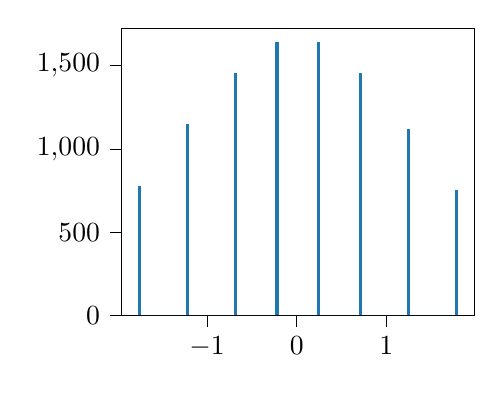
\begin{tikzpicture}

	\definecolor{darkgray176}{RGB}{176,176,176}
	\definecolor{steelblue31119180}{RGB}{31,119,180}
	
	\begin{axis}[
	width=0.5\columnwidth,
	tick align=outside,
	tick pos=left,
	x grid style={darkgray176},
	xmin=-1.95623686313629, xmax=1.98425557613373,
	xtick style={color=black},
	y grid style={darkgray176},
	ymin=0, ymax=1724.1,
	ytick style={color=black}
	]
	\draw[draw=none,fill=steelblue31119180] (axis cs:-1.7771235704422,0) rectangle (axis cs:-1.74130094051361,777);
	\draw[draw=none,fill=steelblue31119180] (axis cs:-1.74130094051361,0) rectangle (axis cs:-1.70547831058502,0);
	\draw[draw=none,fill=steelblue31119180] (axis cs:-1.70547842979431,0) rectangle (axis cs:-1.66965568065643,0);
	\draw[draw=none,fill=steelblue31119180] (axis cs:-1.66965556144714,0) rectangle (axis cs:-1.63383293151855,0);
	\draw[draw=none,fill=steelblue31119180] (axis cs:-1.63383293151855,0) rectangle (axis cs:-1.59801030158997,0);
	\draw[draw=none,fill=steelblue31119180] (axis cs:-1.59801030158997,0) rectangle (axis cs:-1.56218767166138,0);
	\draw[draw=none,fill=steelblue31119180] (axis cs:-1.56218767166138,0) rectangle (axis cs:-1.5263649225235,0);
	\draw[draw=none,fill=steelblue31119180] (axis cs:-1.5263649225235,0) rectangle (axis cs:-1.49054229259491,0);
	\draw[draw=none,fill=steelblue31119180] (axis cs:-1.49054229259491,0) rectangle (axis cs:-1.45471966266632,0);
	\draw[draw=none,fill=steelblue31119180] (axis cs:-1.45471966266632,0) rectangle (axis cs:-1.41889703273773,0);
	\draw[draw=none,fill=steelblue31119180] (axis cs:-1.41889715194702,0) rectangle (axis cs:-1.38307440280914,0);
	\draw[draw=none,fill=steelblue31119180] (axis cs:-1.38307428359985,0) rectangle (axis cs:-1.34725165367126,0);
	\draw[draw=none,fill=steelblue31119180] (axis cs:-1.34725165367126,0) rectangle (axis cs:-1.31142902374268,0);
	\draw[draw=none,fill=steelblue31119180] (axis cs:-1.31142902374268,0) rectangle (axis cs:-1.27560639381409,0);
	\draw[draw=none,fill=steelblue31119180] (axis cs:-1.27560639381409,0) rectangle (axis cs:-1.23978364467621,0);
	\draw[draw=none,fill=steelblue31119180] (axis cs:-1.23978364467621,0) rectangle (axis cs:-1.20396101474762,1151);
	\draw[draw=none,fill=steelblue31119180] (axis cs:-1.20396101474762,0) rectangle (axis cs:-1.16813838481903,0);
	\draw[draw=none,fill=steelblue31119180] (axis cs:-1.16813838481903,0) rectangle (axis cs:-1.13231575489044,0);
	\draw[draw=none,fill=steelblue31119180] (axis cs:-1.13231587409973,0) rectangle (axis cs:-1.09649312496185,0);
	\draw[draw=none,fill=steelblue31119180] (axis cs:-1.09649300575256,0) rectangle (axis cs:-1.06067037582397,0);
	\draw[draw=none,fill=steelblue31119180] (axis cs:-1.06067037582397,0) rectangle (axis cs:-1.02484774589539,0);
	\draw[draw=none,fill=steelblue31119180] (axis cs:-1.02484774589539,0) rectangle (axis cs:-0.989025115966797,0);
	\draw[draw=none,fill=steelblue31119180] (axis cs:-0.989025056362152,0) rectangle (axis cs:-0.953202426433563,0);
	\draw[draw=none,fill=steelblue31119180] (axis cs:-0.953202366828918,0) rectangle (axis cs:-0.91737973690033,0);
	\draw[draw=none,fill=steelblue31119180] (axis cs:-0.91737973690033,0) rectangle (axis cs:-0.881557106971741,0);
	\draw[draw=none,fill=steelblue31119180] (axis cs:-0.881557106971741,0) rectangle (axis cs:-0.845734477043152,0);
	\draw[draw=none,fill=steelblue31119180] (axis cs:-0.845734477043152,0) rectangle (axis cs:-0.809911847114563,0);
	\draw[draw=none,fill=steelblue31119180] (axis cs:-0.809911787509918,0) rectangle (axis cs:-0.774089157581329,0);
	\draw[draw=none,fill=steelblue31119180] (axis cs:-0.774089097976685,0) rectangle (axis cs:-0.738266468048096,0);
	\draw[draw=none,fill=steelblue31119180] (axis cs:-0.738266468048096,0) rectangle (axis cs:-0.702443838119507,0);
	\draw[draw=none,fill=steelblue31119180] (axis cs:-0.702443838119507,0) rectangle (axis cs:-0.666621208190918,1454);
	\draw[draw=none,fill=steelblue31119180] (axis cs:-0.666621148586273,0) rectangle (axis cs:-0.630798518657684,0);
	\draw[draw=none,fill=steelblue31119180] (axis cs:-0.63079845905304,0) rectangle (axis cs:-0.594975829124451,0);
	\draw[draw=none,fill=steelblue31119180] (axis cs:-0.594975829124451,0) rectangle (axis cs:-0.559153199195862,0);
	\draw[draw=none,fill=steelblue31119180] (axis cs:-0.559153199195862,0) rectangle (axis cs:-0.523330569267273,0);
	\draw[draw=none,fill=steelblue31119180] (axis cs:-0.523330509662628,0) rectangle (axis cs:-0.487507879734039,0);
	\draw[draw=none,fill=steelblue31119180] (axis cs:-0.487507820129395,0) rectangle (axis cs:-0.451685190200806,0);
	\draw[draw=none,fill=steelblue31119180] (axis cs:-0.451685190200806,0) rectangle (axis cs:-0.415862560272217,0);
	\draw[draw=none,fill=steelblue31119180] (axis cs:-0.415862560272217,0) rectangle (axis cs:-0.380039930343628,0);
	\draw[draw=none,fill=steelblue31119180] (axis cs:-0.380039870738983,0) rectangle (axis cs:-0.344217240810394,0);
	\draw[draw=none,fill=steelblue31119180] (axis cs:-0.344217240810394,0) rectangle (axis cs:-0.308394610881805,0);
	\draw[draw=none,fill=steelblue31119180] (axis cs:-0.308394551277161,0) rectangle (axis cs:-0.272571921348572,0);
	\draw[draw=none,fill=steelblue31119180] (axis cs:-0.272571891546249,0) rectangle (axis cs:-0.236749261617661,0);
	\draw[draw=none,fill=steelblue31119180] (axis cs:-0.236749231815338,0) rectangle (axis cs:-0.200926601886749,1642);
	\draw[draw=none,fill=steelblue31119180] (axis cs:-0.200926586985588,0) rectangle (axis cs:-0.165103957056999,0);
	\draw[draw=none,fill=steelblue31119180] (axis cs:-0.165103927254677,0) rectangle (axis cs:-0.129281297326088,0);
	\draw[draw=none,fill=steelblue31119180] (axis cs:-0.129281267523766,0) rectangle (axis cs:-0.0934586375951767,0);
	\draw[draw=none,fill=steelblue31119180] (axis cs:-0.0934586077928543,0) rectangle (axis cs:-0.0576359778642654,0);
	\draw[draw=none,fill=steelblue31119180] (axis cs:-0.0576359443366528,0) rectangle (axis cs:-0.0218133144080639,0);
	\draw[draw=none,fill=steelblue31119180] (axis cs:-0.0218132864683867,0) rectangle (axis cs:0.0140093434602022,0);
	\draw[draw=none,fill=steelblue31119180] (axis cs:0.0140093713998795,0) rectangle (axis cs:0.0498320013284683,0);
	\draw[draw=none,fill=steelblue31119180] (axis cs:0.0498320311307907,0) rectangle (axis cs:0.0856546610593796,0);
	\draw[draw=none,fill=steelblue31119180] (axis cs:0.085654690861702,0) rectangle (axis cs:0.121477320790291,0);
	\draw[draw=none,fill=steelblue31119180] (axis cs:0.121477350592613,0) rectangle (axis cs:0.157299980521202,0);
	\draw[draw=none,fill=steelblue31119180] (axis cs:0.157300010323524,0) rectangle (axis cs:0.193122640252113,0);
	\draw[draw=none,fill=steelblue31119180] (axis cs:0.193122670054436,0) rectangle (axis cs:0.228945299983025,0);
	\draw[draw=none,fill=steelblue31119180] (axis cs:0.228945329785347,0) rectangle (axis cs:0.264767944812775,1642);
	\draw[draw=none,fill=steelblue31119180] (axis cs:0.264768004417419,0) rectangle (axis cs:0.300590634346008,0);
	\draw[draw=none,fill=steelblue31119180] (axis cs:0.300590634346008,0) rectangle (axis cs:0.336413264274597,0);
	\draw[draw=none,fill=steelblue31119180] (axis cs:0.336413323879242,0) rectangle (axis cs:0.372235953807831,0);
	\draw[draw=none,fill=steelblue31119180] (axis cs:0.372235953807831,0) rectangle (axis cs:0.40805858373642,0);
	\draw[draw=none,fill=steelblue31119180] (axis cs:0.408058643341064,0) rectangle (axis cs:0.443881273269653,0);
	\draw[draw=none,fill=steelblue31119180] (axis cs:0.443881273269653,0) rectangle (axis cs:0.479703903198242,0);
	\draw[draw=none,fill=steelblue31119180] (axis cs:0.479703933000565,0) rectangle (axis cs:0.515526533126831,0);
	\draw[draw=none,fill=steelblue31119180] (axis cs:0.515526592731476,0) rectangle (axis cs:0.551349222660065,0);
	\draw[draw=none,fill=steelblue31119180] (axis cs:0.551349282264709,0) rectangle (axis cs:0.587171912193298,0);
	\draw[draw=none,fill=steelblue31119180] (axis cs:0.587171912193298,0) rectangle (axis cs:0.622994542121887,0);
	\draw[draw=none,fill=steelblue31119180] (axis cs:0.622994542121887,0) rectangle (axis cs:0.658817172050476,0);
	\draw[draw=none,fill=steelblue31119180] (axis cs:0.658817231655121,0) rectangle (axis cs:0.69463986158371,0);
	\draw[draw=none,fill=steelblue31119180] (axis cs:0.694639921188354,0) rectangle (axis cs:0.730462551116943,1457);
	\draw[draw=none,fill=steelblue31119180] (axis cs:0.730462551116943,0) rectangle (axis cs:0.766285181045532,0);
	\draw[draw=none,fill=steelblue31119180] (axis cs:0.766285181045532,0) rectangle (axis cs:0.802107810974121,0);
	\draw[draw=none,fill=steelblue31119180] (axis cs:0.802107870578766,0) rectangle (axis cs:0.837930500507355,0);
	\draw[draw=none,fill=steelblue31119180] (axis cs:0.837930560112,0) rectangle (axis cs:0.873753190040588,0);
	\draw[draw=none,fill=steelblue31119180] (axis cs:0.873753190040588,0) rectangle (axis cs:0.909575819969177,0);
	\draw[draw=none,fill=steelblue31119180] (axis cs:0.909575819969177,0) rectangle (axis cs:0.945398449897766,0);
	\draw[draw=none,fill=steelblue31119180] (axis cs:0.945398449897766,0) rectangle (axis cs:0.981221079826355,0);
	\draw[draw=none,fill=steelblue31119180] (axis cs:0.981221199035645,0) rectangle (axis cs:1.01704382896423,0);
	\draw[draw=none,fill=steelblue31119180] (axis cs:1.01704382896423,0) rectangle (axis cs:1.05286645889282,0);
	\draw[draw=none,fill=steelblue31119180] (axis cs:1.05286645889282,0) rectangle (axis cs:1.08868908882141,0);
	\draw[draw=none,fill=steelblue31119180] (axis cs:1.08868908882141,0) rectangle (axis cs:1.12451171875,0);
	\draw[draw=none,fill=steelblue31119180] (axis cs:1.12451171875,0) rectangle (axis cs:1.16033446788788,0);
	\draw[draw=none,fill=steelblue31119180] (axis cs:1.16033446788788,0) rectangle (axis cs:1.19615709781647,0);
	\draw[draw=none,fill=steelblue31119180] (axis cs:1.19615709781647,0) rectangle (axis cs:1.23197972774506,0);
	\draw[draw=none,fill=steelblue31119180] (axis cs:1.23197972774506,0) rectangle (axis cs:1.26780235767365,1122);
	\draw[draw=none,fill=steelblue31119180] (axis cs:1.26780223846436,0) rectangle (axis cs:1.30362498760223,0);
	\draw[draw=none,fill=steelblue31119180] (axis cs:1.30362510681152,0) rectangle (axis cs:1.33944773674011,0);
	\draw[draw=none,fill=steelblue31119180] (axis cs:1.33944773674011,0) rectangle (axis cs:1.3752703666687,0);
	\draw[draw=none,fill=steelblue31119180] (axis cs:1.3752703666687,0) rectangle (axis cs:1.41109299659729,0);
	\draw[draw=none,fill=steelblue31119180] (axis cs:1.41109299659729,0) rectangle (axis cs:1.44691574573517,0);
	\draw[draw=none,fill=steelblue31119180] (axis cs:1.44691574573517,0) rectangle (axis cs:1.48273837566376,0);
	\draw[draw=none,fill=steelblue31119180] (axis cs:1.48273837566376,0) rectangle (axis cs:1.51856100559235,0);
	\draw[draw=none,fill=steelblue31119180] (axis cs:1.51856100559235,0) rectangle (axis cs:1.55438363552094,0);
	\draw[draw=none,fill=steelblue31119180] (axis cs:1.55438351631165,0) rectangle (axis cs:1.59020626544952,0);
	\draw[draw=none,fill=steelblue31119180] (axis cs:1.59020638465881,0) rectangle (axis cs:1.6260290145874,0);
	\draw[draw=none,fill=steelblue31119180] (axis cs:1.6260290145874,0) rectangle (axis cs:1.66185164451599,0);
	\draw[draw=none,fill=steelblue31119180] (axis cs:1.66185164451599,0) rectangle (axis cs:1.69767427444458,0);
	\draw[draw=none,fill=steelblue31119180] (axis cs:1.69767427444458,0) rectangle (axis cs:1.73349702358246,0);
	\draw[draw=none,fill=steelblue31119180] (axis cs:1.73349702358246,0) rectangle (axis cs:1.76931965351105,0);
	\draw[draw=none,fill=steelblue31119180] (axis cs:1.76931965351105,0) rectangle (axis cs:1.80514228343964,755);
	\end{axis}
	
\end{tikzpicture}
\label{subfig:aref18dB}
    }
\caption{Learnt joint geometric and probabilistic ASK constellations for M=8.}
\label{fig:arefMASK}
\end{figure}

\end{frame}

\begin{frame}{Overall Performance}
	\centering
	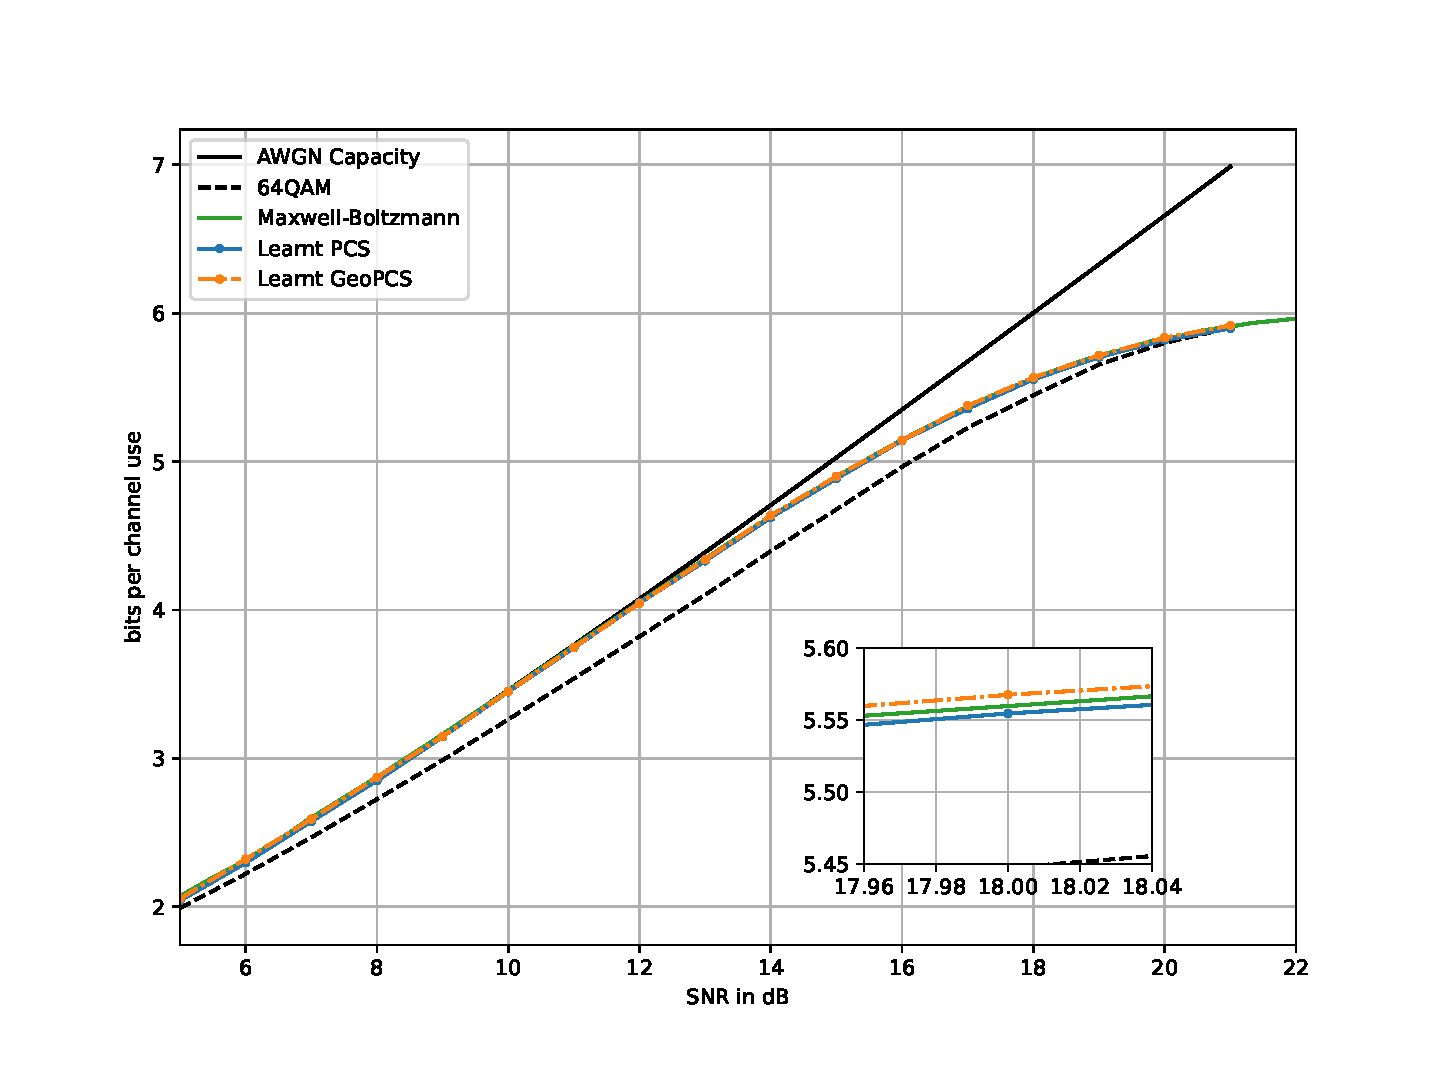
\includegraphics[width=0.75\columnwidth]{aref_gcs.pdf}
	\label{fig:arefPerf}

\end{frame}

\begin{frame}{Conclusions}
\begin{itemize}
\item Both autoencoder proposals show close-to-optimal performance over the AWGN channel.
\item Common keys for success:
	\begin{enumerate}
	\item the choice of the loss function
	\item and correct computation of the gradient w.r.t $P_M$
\end{enumerate}	 
\item The potential of the autoencoder approach is for training over complex channels such as optical fiber.\\
\item Over these channels we expect that they will exhibit different performance.
\item Both \citep{Aref} and \cite{Stark} introduce $\mathbb{H}(X)$ into the loss function. This in turn has the effect of adding a complementary path to the computational graph for computing the gradient w.r.t $P_M$ without backpropagating through the channel model.
\item Training over other channel models is an open research direction with some challenges, such as the limited support of complex data types in the ml frameworks, but promising outcomes
\end{itemize}
\end{frame}

\begin{frame}{Bibliography}
\printbibliography[heading=none]
\end{frame}

%%%%%%%%%%%%%%%%%%%%%%%%%%%%%%%%%%%%%%%%%%%%%%%%%%%%%%%%%%%%%%%%%%%%%%%%%%%%%%%%
\end{document} % !!! NICHT ENTFERNEN !!!
%%%%%%%%%%%%%%%%%%%%%%%%%%%%%%%%%%%%%%%%%%%%%%%%%%%%%%%%%%%%%%%%%%%%%%%%%%%%%%%%

%%% Local Variables:
%%% mode: latex
%%% TeX-master: t
%%% End:
